
% o conteúdo deste arquivo é gerado automaticamente pelo script
% bin/softwares-summary, favor não editar manualmente

\xchapter{Softwares acadêmicos}{Este capítulo ...}
\label{softwares-summary}

\begin{figure}[h]
  \center
  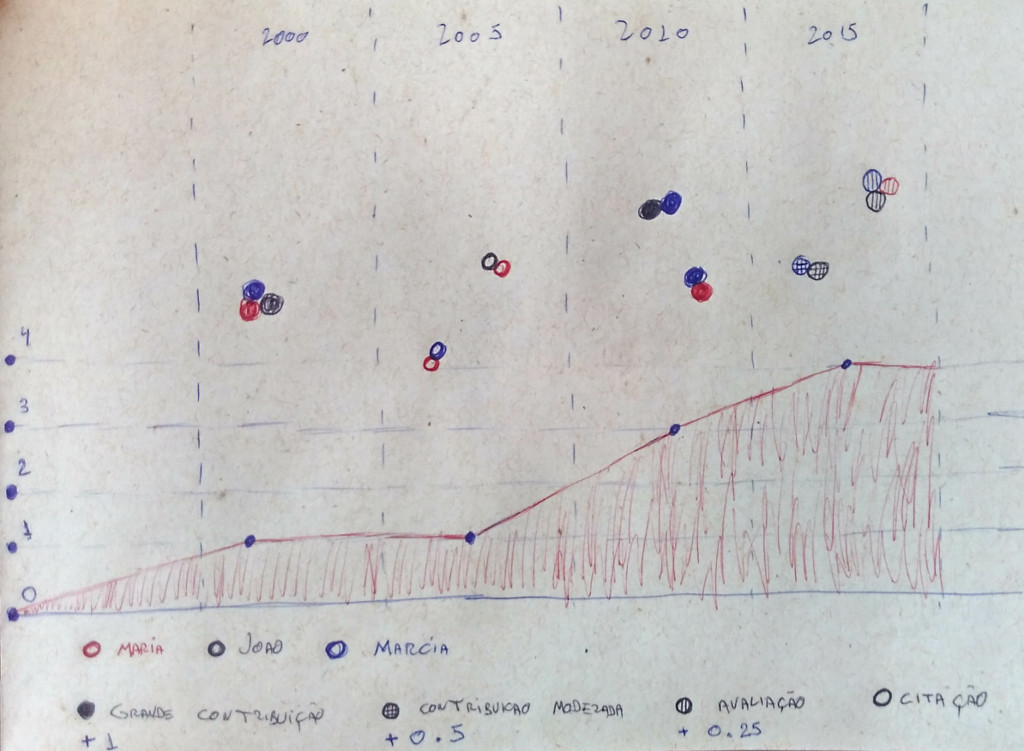
\includegraphics[scale=0.35]{imagens/software-timeline-wireframe.jpg}
  \caption{Protótipo do gráfico com timeline do software}
\end{figure}

\section{2LS - 2nd order Logic Solving}

Análise de terminação para programas C usando resumo interprocedural baseado em modelos
publicado no artigo
Chen Y. H. and David C. and Kroening D. and Schrammel P. and Wachter B.
{\it Synthesising Interprocedural Bit-Precise Termination Proofs (T)}.
2015,
ASE,
disponibilizado em \url{http://svn.cprover.org/wiki/doku.php?id=2ls for program analysis}
como software livre
sob uma licença BSD.

Software com lançamentos ocasionais,
7 versões lançadas
entre 2015 e 2017,
escrito em C++,
uma busca por citações no {\bf IEEE Xplore} por
\texttt{(('2nd order Logic Solving') AND 2LS)}
e no {\bf ACM} por
\texttt{content.ftsec:(2LS) AND (order) AND (Logic) AND (Solving)}
retornou
37 resultados,
nenhum faz referência ao software.


\section{AccessAnalysis}

Cálculo de métricas IGAT e IGAM
publicado no artigo
Zoller C. and Schmolitzky A.
{\it AccessAnalysis: A Tool for Measuring the Appropriateness of Access Modifiers in Java Systems}.
2012,
SCAM,
disponibilizado em \url{http://accessanalysis.sourceforge.net}
como software livre
sob uma licença EPL.

Software considerado obsoleto,
4 versões lançadas
entre 2010 e 2012,
escrito em Java,
uma busca por citações no {\bf IEEE Xplore} por
\texttt{(AccessAnalysis)}
e no {\bf ACM} por
\texttt{content.ftsec:(+AccessAnalysis +Tool +Java +Modifiers)}
retornou
8 resultados,
apenas um faz referência ao software.

\begin{itemize}
\item Zoller C. and Schmolitzky A.
      2012.
      {\it Measuring Inappropriate Generosity with Access Modifiers in Java Systems}.
      Peso da referência: 0
\end{itemize}

Peso total das referências por ano:

\begin{itemize}
\item 2012 = 1
\end{itemize}


\section{APIExample}

Extração de informações de API Java e documentação automática com exemplos
publicado no artigo
Wang L. and Fang L. and Wang L. and Li G. and Xie B. and Yang F.
{\it APIExample: An effective web search based usage example recommendation system for java APIs}.
2011,
ASE,
disponibilizado em \url{http://www.apiexample.com}
mas inacessível em 09/08/2017.

Software sem informações sobre lançamentos ou releases,
uma busca por citações no {\bf IEEE Xplore} por
\texttt{((APIExample) AND Java)}
e no {\bf ACM} por
\texttt{content.ftsec:(+APIExample +Java)}
retornou
16 resultados,
{\bf 3} fazem referência ao software.

\begin{itemize}
\item Zhu Z. and Zou Y. and Jin Y. and Xie B.
      2013.
      {\it Generating API-usage Example for Project Developers}.
      Peso da referência: 0
\item Montandon E. J. and Borges H. and Felix D. and Valente T. M.
      2013.
      {\it Documenting APIs with examples: Lessons learned with the APIMiner platform}.
      Peso da referência: 0
\item Yu H. and Song W. and Mine T.
      2016.
      {\it APIBook: An Effective Approach for Finding APIs}.
      Peso da referência: 0
\end{itemize}

Peso total das referências por ano:

\begin{itemize}
\item 2011 = 1
\item 2013 = 0
\item 2016 = 0
\end{itemize}


\section{BEG - Bandera environment generator}

Criação automática de ambientes para verificação de modelos Java
publicado no artigo
Tkachuk O. and Dwyer B. M. and Pasareanu S. C.
{\it Automated environment generation for software model checking}.
2003,
ASE,
disponibilizado em \url{http://bandera.projects.cs.ksu.edu/}
mas inacessível em 09/08/2017.

Software sem informações sobre lançamentos ou releases,
uma busca por citações no {\bf IEEE Xplore} por
\texttt{(("Bandera environment generator") AND BEG)}
e no {\bf ACM} por
\texttt{content.ftsec:(+"Bandera environment generator" +BEG)}
retornou
10 resultados,
{\bf 8} fazem referência ao software.

\begin{itemize}
\item Dwyer B. M. and Robby and Tkachuk O. and Visser W.
      2004.
      {\it Analyzing interaction orderings with model checking}.
      Peso da referência: 0.25
\item Mutilin V.
      2006.
      {\it Concurrent Testing of Java Components Using Java PathFinder}.
      Peso da referência: 0
\item Tkachuk O. and Rajan P. S.
      2006.
      {\it Application of Automated Environment Generation to Commercial Software}.
      Peso da referência: 0.25
\item Tkachuk O. and Rajan P. S.
      2007.
      {\it Combining Environment Generation and Slicing for Modular Software Model Checking}.
      Peso da referência: 0.25
\item Parizek P. and Plasil F.
      2007.
      {\it Partial Verification of Software Components: Heuristics for Environment Construction}.
      Peso da referência: 0
\item Parizek P. and Plasil F.
      2010.
      {\it Assume-guarantee verification of software components in SOFA 2 framework}.
      Peso da referência: 0
\item Tkachuk O. and Dwyer B. M.
      2010.
      {\it Environment generation for validating event-driven software using model checking}.
      Peso da referência: 0.5
\item Siavashi F. and Truscan D.
      2015.
      {\it Environment Modeling in Model-based Testing: Concepts, Prospects and Research Challenges: A Systematic Literature Review}.
      Peso da referência: 0
\end{itemize}

Peso total das referências por ano:

\begin{itemize}
\item 2003 = 1
\item 2004 = 0.25
\item 2006 = 0.25
\item 2007 = 0.25
\item 2010 = 0.5
\item 2015 = 0
\end{itemize}


\section{ccJava - Class-based Crosscutting Language for Java}

Linguagem orientada a aspectos
publicado no artigo
Ubayashi N. and Sakai A. and Tamai T.
{\it An Aspect-oriented Weaving Mechanism Based on Component and Connector Architecture}.
2007,
ASE,
disponibilizado em \url{http://posl.minnie.ai.kyutech.ac.jp/}
mas inacessível em 09/08/2017.

Software sem informações sobre lançamentos ou releases,
uma busca por citações no {\bf IEEE Xplore} por
\texttt{(ccJava)}
e no {\bf ACM} por
\texttt{content.ftsec:(+ccJava)}
retornou
7 resultados,
{\bf 4} fazem referência ao software.

\begin{itemize}
\item Ubayashi N. and Sakai A. and Tamai T.
      2007.
      {\it An Interface Mechanism for Encapsulating Weaving in Class-based AOP}.
      Peso da referência: 0
\item Ubayashi N. and Sato Y. and Sakai A. and Tamai T.
      2008.
      {\it Alloy-Based Lightweight Verification for Aspect-Oriented Architecture}.
      Peso da referência: 0.5
\item Ubayashi N. and Akatoki H. and Nomura J.
      2009.
      {\it Pointcut-based Architectural Interface for Bridging a Gap Between Design and Implementation}.
      Peso da referência: 0.5
\item Ubayashi N. and Nomura J. and Tamai T.
      2010.
      {\it Archface: A Contract Place Where Architectural Design and Code Meet Together}.
      Peso da referência: 0.5
\end{itemize}

Peso total das referências por ano:

\begin{itemize}
\item 2007 = 1
\item 2008 = 0.5
\item 2009 = 0.5
\item 2010 = 0.5
\end{itemize}


\section{CIVL - Concurrency intermediate verification language}

Framework para verificação de programas concorrentes
publicado no artigo
Zheng M. and Rogers S. M. and Luo Z. and Dwyer B. M. and Siegel F. S.
{\it CIVL: Formal Verification of Parallel Programs}.
2015,
ASE,
disponibilizado em \url{http://vsl.cis.udel.edu/civl/}
como software livre
sob uma licença GPL.

Software com lançamentos frequentes,
36 versões lançadas
entre 2015 e 2017,
escrito em C,
uma busca por citações no {\bf IEEE Xplore} por
\texttt{(('concurrency intermediate verification') AND CIVL)}
e no {\bf ACM} por
\texttt{content.ftsec:(+civl +concurrency +intermediate +verification +language)}
retornou
8 resultados,
{\bf 5} fazem referência ao software.

\begin{itemize}
\item Siegel F. S. and Zheng M. and Luo Z. and Zirkel K. T. and Marianiello V. A. and Edenhofner G. J. and Dwyer B. M. and Rogers S. M.
      2015.
      {\it CIVL: The Concurrency Intermediate Verification Language}.
      Peso da referência: 0
\item L\'{o}pez A. H. and Marques B. R. E. and Martins F. and Ng N. and Santos C. and Vasconcelos T. V. and Yoshida N.
      2015.
      {\it Protocol-based Verification of Message-passing Parallel Programs}.
      Peso da referência: 0
\item Gopalakrishnan G. and Sawaya J.
      2015.
      {\it Achieving Formal Parallel Program Debugging by Incentivizing CS/HPC Collaborative Tool Development}.
      Peso da referência: 0
\item Siegel F. S.
      2017.
      {\it CIVL Solutions to Verifythis 2016 Challenges}.
      Peso da referência: 0
\item Jasper M. and Fecke M. and Steffen B. and Schordan M. and Meijer J. and Pol de van J. and Howar F. and Siegel F. S.
      2017.
      {\it The RERS 2017 Challenge and Workshop (Invited Paper)}.
      Peso da referência: 0
\end{itemize}

Peso total das referências por ano:

\begin{itemize}
\item 2015 = 1
\item 2017 = 0
\end{itemize}


\section{CodeBoost}

Transformação source-to-source para otimização de programas C++
publicado no artigo
Bagge S. O. and Kalleberg T. K. and Haveraaen M. and Visser E.
{\it Design of the CodeBoost transformation system for domain-specific optimisation of C++ programs}.
2003,
SCAM,
disponibilizado em \url{http://codeboost.org}
como software livre
sob uma licença GPL v2.

Software com lançamentos ocasionais,
134 versões lançadas
entre 2000 e 2004,
escrito em C,
uma busca por citações no {\bf IEEE Xplore} por
\texttt{((CodeBoost) AND C++)}
e no {\bf ACM} por
\texttt{content.ftsec:(+CodeBoost +"C++" +Tool)}
retornou
25 resultados,
{\bf 14} fazem referência ao software.

\begin{itemize}
\item L\"{a}mmel R. and Visser E. and Visser J.
      2003.
      {\it Strategic Programming Meets Adaptive Programming}.
      Peso da referência: 0
\item Mernik M. and Heering J. and Sloane M. A.
      2005.
      {\it When and How to Develop Domain-specific Languages}.
      Peso da referência: 0
\item Visser E.
      2005.
      {\it Transformations for abstractions}.
      Peso da referência: 0
\item Schordan M. and Quinlan D.
      2005.
      {\it Specifying transformation sequences as computation on program fragments with an abstract attribute grammar}.
      Peso da referência: 0
\item Quinlan D. and Schordan M. and Vuduc R. and Yi Q.
      2006.
      {\it Annotating user-defined abstractions for optimization}.
      Peso da referência: 0
\item Bravenboer M. and Kalleberg T. K. and Vermaas R. and Visser E.
      2006.
      {\it Stratego/XT 0.16: Components for Transformation Systems}.
      Peso da referência: 0
\item Gottschling P. and Lumsdaine A.
      2008.
      {\it Integrating Semantics and Compilation: Using C++ Concepts to Develop Robust and Efficient Reusable Libraries}.
      Peso da referência: 0
\item Willcock J. J. and Lumsdaine A. and Quinlan J. D.
      2009.
      {\it Reusable, Generic Program Analyses and Transformations}.
      Peso da referência: 0
\item Tang X. and J\"{a}rvi J.
      2010.
      {\it Generic Flow-sensitive Optimizing Transformations in C++ with Concepts}.
      Peso da referência: 0
\item Brown J. K. and Sujeeth K. A. and Lee J. H. and Rompf T. and Chafi H. and Odersky M. and Olukotun K.
      2011.
      {\it A Heterogeneous Parallel Framework for Domain-Specific Languages}.
      Peso da referência: 0
\item Chafi H. and Sujeeth K. A. and Brown J. K. and Lee H. and Atreya R. A. and Olukotun K.
      2011.
      {\it A Domain-specific Approach to Heterogeneous Parallelism}.
      Peso da referência: 0
\item Hong S. and Chafi H. and Sedlar E. and Olukotun K.
      2012.
      {\it Green-Marl: A DSL for Easy and Efficient Graph Analysis}.
      Peso da referência: 0
\item Keep W. A. and Dybvig K. R.
      2013.
      {\it A Nanopass Framework for Commercial Compiler Development}.
      Peso da referência: 0
\item Scherr M. and Chiba S.
      2015.
      {\it Almost First-class Language Embedding: Taming Staged Embedded DSLs}.
      Peso da referência: 0
\end{itemize}

Peso total das referências por ano:

\begin{itemize}
\item 2003 = 1
\item 2005 = 0
\item 2006 = 0
\item 2008 = 0
\item 2009 = 0
\item 2010 = 0
\item 2011 = 0
\item 2012 = 0
\item 2013 = 0
\item 2015 = 0
\end{itemize}


\section{CSL - Composite Symbolic Library}

Verificação de modelos
publicado no artigo
Bultan T. and Yavuz-Kahveci T.
{\it Action Language Verifier}.
2001,
ASE,
disponibilizado em \url{http://www.cs.ucsb.edu/~bultan/composite/}
gratuitamente
sem uma licença definida.

Software sem informações sobre lançamentos ou releases,
escrito em C,
uma busca por citações no {\bf IEEE Xplore} por
\texttt{((((composite) AND bultan) AND Action Language Verifier) OR ("Composite Symbolic Library"))}
e no {\bf ACM} por
\texttt{content.ftsec:(+composite +"Action Language Verifier")}
retornou
14 resultados,
{\bf 5} fazem referência ao software.

\begin{itemize}
\item Fu X. and Bultan T. and Su J.
      2004.
      {\it Realizability of conversation protocols with message contents}.
      Peso da referência: 0
\item Zhang D. and Cleaveland R.
      2005.
      {\it Efficient Temporal-logic Query Checking for Presburger Systems}.
      Peso da referência: 0
\item Bultan T. and Heitmeyer C.
      2006.
      {\it Analyzing Tabular Requirements Specifications Using Infinite State Model Checking}.
      Peso da referência: 0.25
\item Yang Z. and Wang C. and Gupta A. and Ivancic F.
      2006.
      {\it Mixed Symbolic Representations for Model Checking Software Programs}.
      Peso da referência: 0.5
\item Yang Z. and Wang C. and Gupta A. and Ivan\v{c}i\'{c} F.
      2009.
      {\it Model Checking Sequential Software Programs via Mixed Symbolic Analysis}.
      Peso da referência: 0.25
\end{itemize}

Peso total das referências por ano:

\begin{itemize}
\item 2001 = 1
\item 2004 = 0
\item 2005 = 0
\item 2006 = 0.75
\item 2009 = 0.25
\end{itemize}


\section{CPA+ - Configurable program analysis with dynamic precision adjustment}

Análise configurável de programa com ajuste dinâmico de precisão
publicado no artigo
Beyer D. and Henzinger A. T. and Theoduloz G.
{\it Program Analysis with Dynamic Precision Adjustment}.
2008,
ASE,
disponibilizado em \url{http://www.cs.sfu.ca/~dbeyer/blast_cpaplus/}
mas inacessível em 09/08/2017.

Software sem informações sobre lançamentos ou releases,
uma busca por citações no {\bf IEEE Xplore} por
\texttt{(('program analysis') AND cpa+)}
e no {\bf ACM} por
\texttt{content.ftsec:(+cpa +dbeyer)}
retornou
8 resultados,
{\bf 4} fazem referência ao software.

\begin{itemize}
\item Beyer D. and Keremoglu E. M. and Wendler P.
      2010.
      {\it Predicate Abstraction with Adjustable-block Encoding}.
      Peso da referência: 0.5
\item Beyer D. and Henzinger A. T. and Keremoglu E. M. and Wendler P.
      2012.
      {\it Conditional Model Checking: A Technique to Pass Information Between Verifiers}.
      Peso da referência: 0.5
\item Beyer D. and L\"{o}we S. and Novikov E. and Stahlbauer A. and Wendler P.
      2013.
      {\it Precision Reuse for Efficient Regression Verification}.
      Peso da referência: 0.5
\item Beyer D. and Dangl M. and Dietsch D. and Heizmann M. and Stahlbauer A.
      2015.
      {\it Witness Validation and Stepwise Testification Across Software Verifiers}.
      Peso da referência: 0.5
\end{itemize}

Peso total das referências por ano:

\begin{itemize}
\item 2008 = 1
\item 2010 = 0.5
\item 2012 = 0.5
\item 2013 = 0.5
\item 2015 = 0.5
\end{itemize}


\section{CSeq}

Transformação source-to-source para programas C concorrentes
publicado no artigo
Fischer B. and Inverso O. and Parlato G.
{\it CSeq: A concurrency pre-processor for sequential C verification tools}.
2013,
ASE,
disponibilizado em \url{http://users.ecs.soton.ac.uk/gp4/cseq/files/cseq-0.5.zip}
como software livre
sob uma licença BSD.

Software sem informações sobre lançamentos ou releases,
escrito em C,
uma busca por citações no {\bf IEEE Xplore} por
\texttt{((CSeq) AND soton)}
e no {\bf ACM} por
\texttt{content.ftsec:(+cseq +sequential +verification +tool)}
retornou
16 resultados,
{\bf 4} fazem referência ao software.

\begin{itemize}
\item Inverso O. and Nguyen L. T. and Fischer B. and Torre L. S. and Parlato G.
      2015.
      {\it Lazy-CSeq: A Context-Bounded Model Checking Tool for Multi-threaded C-Programs}.
      Peso da referência: 0.5
\item Bouajjani A. and Emmi M. and Enea C. and Hamza J.
      2015.
      {\it Tractable Refinement Checking for Concurrent Objects}.
      Peso da referência: 0.25
\item Mayer M. and Madhavan R.
      2016.
      {\it A Scala Library for Testing Student Assignments on Concurrent Programming}.
      Peso da referência: 0
\item Tomasco E. and Nguyen L. T. and Inverso O. and Fischer B. and L. Torre S. and Parlato G.
      2016.
      {\it Lazy Sequentialization for TSO and PSO via Shared Memory Abstractions}.
      Peso da referência: 0.25
\end{itemize}

Peso total das referências por ano:

\begin{itemize}
\item 2013 = 1
\item 2015 = 0.75
\item 2016 = 0.25
\end{itemize}


\section{DDVerify}

Verificação de Linux drivers através de checagem de modelos
publicado no artigo
Witkowski T. and Blanc N. and Kroening D. and Weissenbacher G.
{\it Model Checking Concurrent Linux Device Drivers}.
2007,
ASE,
disponibilizado em \url{http://www.verify.ethz.ch/ddverify}
mas inacessível em 09/08/2017.

Software sem informações sobre lançamentos ou releases,
uma busca por citações no {\bf IEEE Xplore} por
\texttt{(DDVerify)}
e no {\bf ACM} por
\texttt{content.ftsec:(+DDVerify)}
retornou
4 resultados,
{\bf 2} fazem referência ao software.

\begin{itemize}
\item Blanc N. and Kroening D.
      2008.
      {\it Race Analysis for SystemC Using Model Checking}.
      Peso da referência: 0
\item Dileep P. K. and Raghavendra A. and Suman M. and Devesh G. and Srikanth V. S.
      2014.
      {\it Rules based automatic Linux Device Driver Verifier And Code Assistance}.
      Peso da referência: 0
\end{itemize}

Peso total das referências por ano:

\begin{itemize}
\item 2007 = 1
\item 2008 = 0
\item 2014 = 0
\end{itemize}


\section{Derailer}

Localização de falhas de segurança em aplicações web
publicado no artigo
Near P. J. and Jackson D.
{\it Derailer: Interactive Security Analysis for Web Applications}.
2014,
ASE,
disponibilizado em \url{http://people.csail.mit.edu/jnear/derailer}
como software livre
sob uma licença GPL v3.

Software considerado obsoleto,
2 versões lançadas
entre 2013 e 2014,
escrito em Ruby,
uma busca por citações no {\bf IEEE Xplore} por
\texttt{((Derailer) AND jnear)}
e no {\bf ACM} por
\texttt{content.ftsec:(+Derailer +analysis +security +web +tool +bugs +ruby)}
retornou
7 resultados,
apenas um faz referência ao software.

\begin{itemize}
\item Near P. J. and Jackson D.
      2016.
      {\it Finding Security Bugs in Web Applications Using a Catalog of Access Control Patterns}.
      Peso da referência: 0
\end{itemize}

Peso total das referências por ano:

\begin{itemize}
\item 2014 = 1
\item 2016 = 0
\end{itemize}


\section{Diagnosys}

Construção de interfaces de debug para o kernel Linux
publicado no artigo
Bissyandé F. T. and Réveillère L. and Lawall L. J. and Muller G.
{\it Diagnosys: automatic generation of a debugging interface to the Linux kernel}.
2012,
ASE,
disponibilizado em \url{http://momentum.labri.fr/projects/diagnosys}
mas inacessível em 09/08/2017.

Software sem informações sobre lançamentos ou releases,
uma busca por citações no {\bf IEEE Xplore} por
\texttt{((Diagnosys) AND debugging)}
e no {\bf ACM} por
\texttt{content.ftsec:(+"Diagnosys tool" +Debugging +Linux +"device drivers")}
retornou
9 resultados,
nenhum faz referência ao software.


\section{DOMPLETION}

Sugestão de código javascript
publicado no artigo
Bajaj K. and Pattabiraman K. and Mesbah A.
{\it Dompletion: DOM-aware JavaScript Code Completion}.
2014,
ASE,
disponibilizado em \url{https://github.com/saltlab/dompletion}
gratuitamente
sem uma licença definida.

Software sem informações sobre lançamentos ou releases,
escrito em Javascript,
uma busca por citações no {\bf IEEE Xplore} por
\texttt{content.ftsec:(+dompletion +JavaScript)}
e no {\bf ACM} por
\texttt{((dompletion) AND JavaScript)}
retornou
2 resultados,
apenas um faz referência ao software.

\begin{itemize}
\item Bajaj K. and Pattabiraman K. and Mesbah A.
      2015.
      {\it LED: Tool for Synthesizing Web Element Locators}.
      Peso da referência: 0
\end{itemize}

Peso total das referências por ano:

\begin{itemize}
\item 2014 = 1
\item 2015 = 0
\end{itemize}


\section{DRC - Dangling Reference Checker}

Análise estática para detecção de referências inválidas em código dinâmico PHP
publicado no artigo
Nguyen V. H. and Nguyen A. H. and Nguyen T. T. and Nguyen T. A. and Nguyen N. T.
{\it Dangling references in multi-configuration and dynamic PHP-based Web applications}.
2013,
ASE,
disponibilizado em \url{http://home.engineering.iastate.edu/~hungnv/Research/DRC}
mas inacessível em 09/08/2017.

Software sem informações sobre lançamentos ou releases,
uma busca por citações no {\bf IEEE Xplore} por
\texttt{(DRC Dangling Reference Checker)}
e no {\bf ACM} por
\texttt{content.ftsec:(+DRC +Dangling +Reference)}
retornou
19 resultados,
{\bf 4} fazem referência ao software.

\begin{itemize}
\item Nguyen V. H. and Nguyen A. H. and Nguyen T. T. and Nguyen N. T.
      2013.
      {\it DRC: A detection tool for dangling references in PHP-based web applications}.
      Peso da referência: 0
\item Eshkevari L. and Antoniol G. and Cordy R. J. and D. Penta M.
      2014.
      {\it Identifying and Locating Interference Issues in PHP Applications: The Case of WordPress}.
      Peso da referência: 0
\item Nguyen V. H. and K\"{a}stner C. and Nguyen N. T.
      2014.
      {\it Building Call Graphs for Embedded Client-side Code in Dynamic Web Applications}.
      Peso da referência: 0
\item Nguyen V. H. and K\"{a}stner C. and Nguyen N. T.
      2015.
      {\it Cross-language Program Slicing for Dynamic Web Applications}.
      Peso da referência: 0
\end{itemize}

Peso total das referências por ano:

\begin{itemize}
\item 2013 = 1
\item 2014 = 0
\item 2015 = 0
\end{itemize}


\section{e-munity}

Verificação de segurança
publicado no artigo
Tlili S. and Fernandez M. J. and Belghith A. and Dridi B. and Hidouri S.
{\it Scalable Security Verification of Software at Compile Time}.
2014,
SCAM,
disponibilizado em \url{http://sourceforge.net/p/emunity/code/ci/master/tree/}
gratuitamente
sem uma licença definida.

Software sem informações sobre lançamentos ou releases,
escrito em C,
uma busca por citações no {\bf IEEE Xplore} por
\texttt{(e-munity)}
e no {\bf ACM} por
\texttt{content.ftsec:(+"e-munity")}
retornou
1 resultados,
nenhum faz referência ao software.


\section{EJB Interceptor Analyzer}

Criação de diagramas de sequência
publicado no artigo
Roubtsov S. and Serebrenik A. and Mazoyer A. and Brand d. v. M.
{\it I2SD: Reverse Engineering Sequence Diagrams from Enterprise Java Beans with Interceptors}.
2011,
SCAM,
disponibilizado em \url{https://www.dropbox.com/s/glhg8any43lccgm/EJB.zip}
gratuitamente
sem uma licença definida.

Software sem informações sobre lançamentos ou releases,
escrito em Java,
uma busca por citações no {\bf IEEE Xplore} por
\texttt{(((I2SD) AND EJB) AND Java)}
e no {\bf ACM} por
\texttt{content.ftsec:(+I2SD +Java)}
retornou
5 resultados,
{\bf 2} fazem referência ao software.

\begin{itemize}
\item Sutii A. and Roubtsov S. and Serebrenik A.
      2013.
      {\it Detecting dependencies in Enterprise JavaBeans with SQuAVisiT}.
      Peso da referência: 0
\item Mushtaq Z. and Rasool G. and Shehzad B.
      2017.
      {\it Multilingual Source Code Analysis: A Systematic Literature Review}.
      Peso da referência: 0.25
\end{itemize}

Peso total das referências por ano:

\begin{itemize}
\item 2011 = 1
\item 2013 = 0
\item 2017 = 0.25
\end{itemize}


\section{Error Prone}

Localização de bugs em código Java construído em cima do compilador javac
publicado no artigo
Aftandilian E. and Sauciuc R. and Priya S. and Krishnan S.
{\it Building Useful Program Analysis Tools Using an Extensible Java Compiler}.
2012,
SCAM,
disponibilizado em \url{http://code.google.com/p/error-prone}
como software livre
sob uma licença Apache License v2.0.

Software com lançamentos frequentes,
22 versões lançadas
entre 2015 e 2017,
escrito em Java,
uma busca por citações no {\bf IEEE Xplore} por
\texttt{((((('error-prone tool') AND Analysis) AND 'java compiler') AND 'error checks') AND javac)}
e no {\bf ACM} por
\texttt{content.ftsec:(+"error-prone" +tool +javac +analysis +"java compiler")}
retornou
47 resultados,
apenas um faz referência ao software.

\begin{itemize}
\item Sadowski C. and Gogh v. J. and Jaspan C. and Söderberg E. and Winter C.
      2015.
      {\it Tricorder: Building a Program Analysis Ecosystem}.
      Peso da referência: 0.25
\end{itemize}

Peso total das referências por ano:

\begin{itemize}
\item 2012 = 1
\item 2015 = 0.25
\end{itemize}


\section{ESBMC - Efficient SMT-Based Context-Bounded Model Checker}

Verificação de modelos
publicado no artigo
Cordeiro L. and Fischer B. and Marques-Silva J.
{\it SMT-Based Bounded Model Checking for Embedded ANSI-C Software}.
2009,
ASE,
disponibilizado em \url{http://users.ecs.soton.ac.uk/lcc08r/esbmc/}
mas inacessível em 09/08/2017.

Software sem informações sobre lançamentos ou releases,
uma busca por citações no {\bf IEEE Xplore} por
\texttt{(ESBMC)}
e no {\bf ACM} por
\texttt{content.ftsec:(+ESBMC)}
retornou
50 resultados,
{\bf 41} fazem referência ao software.

\begin{itemize}
\item Cordeiro L. and Fischer B. and Marques-Silva J.
      2010.
      {\it Continuous Verification of Large Embedded Software Using SMT-Based Bounded Model Checking}.
      Peso da referência: 0.25
\item Barreto R. and Cordeiro L. and Fischer B.
      2011.
      {\it Verifying Embedded C Software with Timing Constraints Using an Untimed Bounded Model Checker}.
      Peso da referência: 0.5
\item Behrend J. and Lettnin D. and Heckeler P. and Ruf J. and Kropf T. and Rosenstiel W.
      2011.
      {\it Scalable hybrid verification for embedded software}.
      Peso da referência: 0.25
\item Cordeiro L. and Fischer B.
      2011.
      {\it Verifying Multi-threaded Software Using Smt-based Context-bounded Model Checking}.
      Peso da referência: 0.25
\item Gharehbaghi M. A. and Fujita M.
      2012.
      {\it Transaction-based post-silicon debug of many-core System-on-Chips}.
      Peso da referência: 0.25
\item Abdulla A. P. and Atig F. M. and Rezine O. and Stenman J.
      2012.
      {\it Multi-pushdown systems with budgets}.
      Peso da referência: 0.25
\item Banerjee K. and Prabhu S. M. and Dasgupta P.
      2013.
      {\it Debugging Assertion Failures in Software Controllers Using a Reference Model}.
      Peso da referência: 0
\item Ramalho M. and Freitas M. and Sousa F. and Marques H. and Cordeiro L. and Fischer B.
      2013.
      {\it SMT-Based Bounded Model Checking of C++ Programs}.
      Peso da referência: 0.5
\item Fischer B. and Inverso O. and Parlato G.
      2013.
      {\it CSeq: A Concurrency Pre-processor for Sequential C Verification Tools}.
      Peso da referência: 0
\item Falke S. and Merz F. and Sinz C.
      2013.
      {\it The bounded model checker LLBMC}.
      Peso da referência: 0.25
\item Wachter B. and Kroening D. and Ouaknine J.
      2013.
      {\it Verifying multi-threaded software with impact}.
      Peso da referência: 0.25
\item Cho Y. C. and D'Silva V. and Song D.
      2013.
      {\it BLITZ: Compositional Bounded Model Checking for Real-world Programs}.
      Peso da referência: 0.25
\item Bessa d. V. I. and Ismail I. H. and Cordeiro C. L. and Filho C. E. J.
      2014.
      {\it Verification of Delta Form Realization in Fixed-Point Digital Controllers Using Bounded Model Checking}.
      Peso da referência: 0.25
\item Behrend J. and Gruenhage A. and Schroeder D. and Lettnin D. and Ruf J. and Kropf T. and Rosenstiel W.
      2014.
      {\it Optimized hybrid verification of embedded software}.
      Peso da referência: 0.25
\item G\"{u}nther H. and Weissenbacher G.
      2014.
      {\it Incremental Bounded Software Model Checking}.
      Peso da referência: 0.25
\item Januario P. A. F. and Cordeiro C. L. and Lucena d. F. V. and Filho L. d. B. E.
      2014.
      {\it BMCLua: Verification of Lua programs in digital TV interactive applications}.
      Peso da referência: 0.5
\item Cordy M. and Heymans P. and Legay A. and Schobbens P. and Dawagne B. and Leucker M.
      2014.
      {\it Counterexample Guided Abstraction Refinement of Product-line Behavioural Models}.
      Peso da referência: 0
\item Thomson P. and Donaldson F. A. and Betts A.
      2014.
      {\it Concurrency Testing Using Schedule Bounding: An Empirical Study}.
      Peso da referência: 0.25
\item Gupta A. and Henzinger A. T. and Radhakrishna A. and Samanta R. and Tarrach T.
      2015.
      {\it Succinct Representation of Concurrent Trace Sets}.
      Peso da referência: 0
\item Rocha H. and Ismail H. and Cordeiro L. and Barreto R.
      2015.
      {\it Model Checking Embedded C Software Using k-Induction and Invariants}.
      Peso da referência: 0.5
\item Sousa M. R. F. and Cordeiro C. L. and Filho L. de B. E.
      2015.
      {\it Bounded model checking of C++ programs based on the Qt framework}.
      Peso da referência: 0.5
\item Trindade A. and Ismail H. and Cordeiro L.
      2015.
      {\it Applying Multi-core Model Checking to Hardware-Software Partitioning in Embedded Systems}.
      Peso da referência: 0.5
\item Chabot M. and Mazet K. and Pierre L.
      2015.
      {\it Automatic and configurable instrumentation of C programs with temporal assertion checkers}.
      Peso da referência: 0
\item Inverso O. and Nguyen L. T. and Fischer B. and Torre L. S. and Parlato G.
      2015.
      {\it Lazy-CSeq: A Context-Bounded Model Checking Tool for Multi-threaded C-Programs}.
      Peso da referência: 0
\item Darke P. and Chimdyalwar B. and Venkatesh R. and Shrotri U. and Metta R.
      2015.
      {\it Over-approximating Loops to Prove Properties Using Bounded Model Checking}.
      Peso da referência: 0.25
\item Alves S. d. H. E. and Cordeiro C. L. and Filho L. d. B. E.
      2015.
      {\it Fault Localization in Multi-threaded C Programs Using Bounded Model Checking}.
      Peso da referência: 0.25
\item Araújo R. and Bessa I. and Cordeiro C. L. and Filho C. E. J.
      2016.
      {\it SMT-based Verification Applied to Non-convex Optimization Problems}.
      Peso da referência: 0.25
\item Gao M. and He L. and Majumdar R. and Wang Z.
      2016.
      {\it LLSPLAT: Improving Concolic Testing by Bounded Model Checking}.
      Peso da referência: 0
\item Bentes L. and Rocha H. and Valentin E. and Barreto R.
      2016.
      {\it JFORTES: Java Formal Unit TESt Generation}.
      Peso da referência: 0
\item Pereira P. and Albuquerque H. and Marques H. and Silva I. and Carvalho C. and Cordeiro L. and Santos V. and Ferreira R.
      2016.
      {\it Verifying CUDA Programs Using SMT-based Context-bounded Model Checking}.
      Peso da referência: 0.5
\item Xie X. and Chen B. and Liu Y. and Le W. and Li X.
      2016.
      {\it Proteus: Computing Disjunctive Loop Summary via Path Dependency Analysis}.
      Peso da referência: 0
\item Paludo R. and Lettnin D.
      2016.
      {\it A methodology for early functional verification of embedded software combining virtual platforms and bounded model checking}.
      Peso da referência: 0.25
\item Cordeiro C. L. and d. L. Filho B. E.
      2016.
      {\it SMT-Based Context-Bounded Model Checking for Embedded Systems: Challenges and Future Trends}.
      Peso da referência: 0
\item Kroening D. and Poetzl D. and Schrammel P. and Wachter B.
      2016.
      {\it Sound static deadlock analysis for C/Pthreads}.
      Peso da referência: 0
\item Monteiro R. F.
      2016.
      {\it Bounded Model Checking of State-space Digital Systems: The Impact of Finite Word-length Effects on the Implementation of Fixed-point Digital Controllers Based on State-space Modeling}.
      Peso da referência: 0
\item Zhang X. and Yang Z. and Zheng Q. and Hao Y. and Liu P. and Yu L. and Fan M. and Liu T.
      2016.
      {\it Debugging Multithreaded Programs as if They Were Sequential}.
      Peso da referência: 0.25
\item Beyer D. and Dangl M. and Dietsch D. and Heizmann M.
      2016.
      {\it Correctness Witnesses: Exchanging Verification Results Between Verifiers}.
      Peso da referência: 0
\item Chaves L. and Bessa I. and Cordeiro L. and Kroening D. and Lima E.
      2017.
      {\it Verifying Digital Systems with MATLAB}.
      Peso da referência: 0
\item Zheng X. and Julien C. and Podorozhny R. and Cassez F. and Rakotoarivelo T.
      2017.
      {\it Efficient and Scalable Runtime Monitoring for Cyber--Physical System}.
      Peso da referência: 0
\item Zhang X.
      2017.
      {\it Debugging Multithreaded Programs Using Symbolic Analysis}.
      Peso da referência: 0.25
\item Zhang X. and Yang Z. and Zheng Q. and Liu P. and Chang J. and Hao Y. and Liu T.
      2017.
      {\it Automated Testing of Definition-Use Data Flow for Multithreaded Programs}.
      Peso da referência: 0.25
\end{itemize}

Peso total das referências por ano:

\begin{itemize}
\item 2009 = 1
\item 2010 = 0.25
\item 2011 = 1
\item 2012 = 0.5
\item 2013 = 1.25
\item 2014 = 1.5
\item 2015 = 2
\item 2016 = 1.25
\item 2017 = 0.5
\end{itemize}


\section{ETXL}

Transformação de código
publicado no artigo
Thurston D. A. and Cordy R. J.
{\it Evolving TXL}.
2006,
SCAM,
disponibilizado em \url{http://www.cs.queensu.ca/home/thurston/etxl}
mas inacessível em 09/08/2017.

Software sem informações sobre lançamentos ou releases,
uma busca por citações no {\bf IEEE Xplore} por
\texttt{(((ETXL) AND source) AND transformation)}
e no {\bf ACM} por
\texttt{content.ftsec:(+ETXL)}
retornou
10 resultados,
nenhum faz referência ao software.


\section{FaultBuster}

Refatoração de code smells
publicado no artigo
Szőke G. and Nagy C. and Fülöp J. L. and Ferenc R. and Gyimóthy T.
{\it FaultBuster: An automatic code smell refactoring toolset}.
2015,
SCAM,
disponibilizado em \url{http://www.sed.inf.u-szeged.hu/FaultBuster}
gratuitamente
sob uma licença de demonstração.

Software sem informações sobre lançamentos ou releases,
uma busca por citações no {\bf IEEE Xplore} por
\texttt{(FaultBuster)}
e no {\bf ACM} por
\texttt{content.ftsec:(+FaultBuster)}
retornou
4 resultados,
nenhum faz referência ao software.


\section{Flowgen}

Criação automática de grafos UML
publicado no artigo
Kosower A. D. and Lopez-Villarejo J. J. and Roubtsov S.
{\it Flowgen: Flowchart-Based Documentation Framework for C++}.
2014,
SCAM,
disponibilizado em \url{https://github.com/jlopezvi/Flowgen}
como software livre
sob uma licença GPL v3.

Software sem informações sobre lançamentos ou releases,
escrito em Python,
uma busca por citações no {\bf IEEE Xplore} por
\texttt{((Flowgen) AND C++)}
e no {\bf ACM} por
\texttt{content.ftsec:(+Flowgen)}
retornou
8 resultados,
{\bf 2} fazem referência ao software.

\begin{itemize}
\item Georget L. and Tronel F. and Tong T. V. V.
      2015.
      {\it Kayrebt: An activity diagram extraction and visualization toolset designed for the Linux codebase}.
      Peso da referência: 0
\item Moser M. and Pichler J.
      2016.
      {\it Documentation Generation from Annotated Source Code of Scientific Software}.
      Peso da referência: 0
\end{itemize}

Peso total das referências por ano:

\begin{itemize}
\item 2014 = 1
\item 2015 = 0
\item 2016 = 0
\end{itemize}


\section{GRT - Guided Random Testing}

Geração automática de testes
publicado no artigo
Ma L. and Artho C. and Zhang C. and Sato H. and Gmeiner J. and Ramler R.
{\it GRT: Program-Analysis-Guided Random Testing (T)}.
2015,
ASE,
disponibilizado em \url{http://www.sites.google.com/site/grtprojectut/download}
mas inacessível em 09/08/2017.

Software sem informações sobre lançamentos ou releases,
uma busca por citações no {\bf IEEE Xplore} por
\texttt{((GRT) AND "Guided Random Testing")}
e no {\bf ACM} por
\texttt{content.ftsec:(+GRT) +"Guided Random Testing")}
retornou
13 resultados,
{\bf 7} fazem referência ao software.

\begin{itemize}
\item Chiang W. and Gopalakrishnan G. and Rakamaric Z. and Solovyev A.
      2014.
      {\it Efficient Search for Inputs Causing High Floating-point Errors}.
      Peso da referência: 0
\item Ma L. and Artho C. and Zhang C. and Sato H. and Hagiya M. and Tanabe Y. and Yamamoto M.
      2015.
      {\it GRT at the SBST 2015 Tool Competition}.
      Peso da referência: 0
\item Artho C. and Ma L.
      2016.
      {\it Classification of Randomly Generated Test Cases}.
      Peso da referência: 0.25
\item Ma L. and Zhang C. and Yu B. and Zhao J.
      2016.
      {\it Retrofitting automatic testing through library tests reusing}.
      Peso da referência: 0.5
\item Arcuri A. and Fraser G. and Just R.
      2017.
      {\it Private API Access and Functional Mocking in Automated Unit Test Generation}.
      Peso da referência: 0
\item Panichella A. and Kifetew F. and Tonella P.
      2017.
      {\it Automated Test Case Generation as a Many-Objective Optimisation Problem with Dynamic Selection of the Targets}.
      Peso da referência: 0
\item Artho C. and Gros Q. and Rousset G. and Banzai K. and Ma L. and Kitamura T. and Hagiya M. and Tanabe Y. and Yamamoto M.
      2017.
      {\it Model-Based API Testing of Apache ZooKeeper}.
      Peso da referência: 0.25
\end{itemize}

Peso total das referências por ano:

\begin{itemize}
\item 2014 = 0
\item 2015 = 1
\item 2016 = 0.75
\item 2017 = 0.25
\end{itemize}


\section{GUIZMO}

Inferência de layout
publicado no artigo
S. Ram\'{o}n \'{O}scar and S. Cuadrado J. and G. Molina J.
{\it Model-driven Reverse Engineering of Legacy Graphical User Interfaces}.
2010,
ASE,
disponibilizado em \url{http://modelum.es/trac/guizmo/}
como software livre
sob uma licença Apache License v2.0.

Software sem informações sobre lançamentos ou releases,
escrito em Java,
uma busca por citações no {\bf IEEE Xplore} por
\texttt{(guizmo)}
e no {\bf ACM} por
\texttt{content.ftsec:(+guizmo)}
retornou
0 resultados,
nenhum faz referência ao software.


\section{GumTree}

Comparação de mudanças
publicado no artigo
Falleri J. and Morandat F. and Blanc X. and Martinez M. and Monperrus M.
{\it Fine-grained and Accurate Source Code Differencing}.
2014,
ASE,
disponibilizado em \url{https://github.com/jrfaller/gumtree}
como software livre
sob uma licença LGPL v3.

Software com lançamentos ocasionais,
3 versões lançadas
entre 2013 e 2015,
escrito em Java,
uma busca por citações no {\bf IEEE Xplore} por
\texttt{((GumTree) AND tool)}
e no {\bf ACM} por
\texttt{content.ftsec:(+GumTree +tool)}
retornou
37 resultados,
{\bf 17} fazem referência ao software.

\begin{itemize}
\item Gao Q. and Zhang H. and Wang J. and Xiong Y. and Zhang L. and Mei H.
      2015.
      {\it Fixing Recurring Crash Bugs via Analyzing Q\&A Sites (T)}.
      Peso da referência: 0.25
\item Zimmerman K. and Rupakheti R. C.
      2015.
      {\it An Automated Framework for Recommending Program Elements to Novices (N)}.
      Peso da referência: 0
\item Dotzler G. and Philippsen M.
      2016.
      {\it Move-optimized source code tree differencing}.
      Peso da referência: 0.5
\item Ahmed I. and Gopinath R. and Brindescu C. and Groce A. and Jensen C.
      2016.
      {\it Can Testedness Be Effectively Measured?}.
      Peso da referência: 0.25
\item Nguyen T. A. and Hilton M. and Codoban M. and Nguyen A. H. and Mast L. and Rademacher E. and Nguyen N. T. and Dig D.
      2016.
      {\it API Code Recommendation Using Statistical Learning from Fine-grained Changes}.
      Peso da referência: 0.25
\item Le D. B. X. and Lo D. and Goues L. C.
      2016.
      {\it History Driven Program Repair}.
      Peso da referência: 0.25
\item Kreutzer P. and Dotzler G. and Ring M. and Eskofier M. B. and Philippsen M.
      2016.
      {\it Automatic Clustering of Code Changes}.
      Peso da referência: 0
\item Hanam Q. and Brito M. de S. F. and Mesbah A.
      2016.
      {\it Discovering Bug Patterns in JavaScript}.
      Peso da referência: 0.25
\item Koyuncu A. and Bissyand{\'e} F. T. and Kim D. and Klein J. and Monperrus M. and L. Traon Y.
      2017.
      {\it Impact of Tool Support in Patch Construction}.
      Peso da referência: 0.25
\item Macho C. and Mcintosh S. and Pinzger M.
      2017.
      {\it Extracting Build Changes with BuildDiff}.
      Peso da referência: 0.25
\item Le D. X. and Chu D. and Lo D. and L. Goues C. and Visser W.
      2017.
      {\it S3: Syntax- and Semantic-guided Repair Synthesis via Programming by Examples}.
      Peso da referência: 0.25
\item rempel p. and Mader P.
      2017.
      {\it Preventing Defects: The Impact of Requirements Traceability Completeness on Software Quality}.
      Peso da referência: 0.25
\item Tan H. S. and Yi J. and Yulis and Mechtaev S. and Roychoudhury A.
      2017.
      {\it Codeflaws: A Programming Competition Benchmark for Evaluating Automated Program Repair Tools}.
      Peso da referência: 0.5
\item Soetens D. Q. and Robbes R. and Demeyer S.
      2017.
      {\it Changes As First-Class Citizens: A Research Perspective on Modern Software Tooling}.
      Peso da referência: 0
\item Stevens R. and Roover D. C.
      2017.
      {\it Extracting executable transformations from distilled code changes}.
      Peso da referência: 0
\item Yi J. and Ahmed Z. U. and Karkare A. and Tan H. S. and Roychoudhury A.
      2017.
      {\it A Feasibility Study of Using Automated Program Repair for Introductory Programming Assignments}.
      Peso da referência: 0.25
\item Laverdière A. M. and Merlo E.
      2017.
      {\it Computing counter-examples for privilege protection losses using security models}.
      Peso da referência: 0
\end{itemize}

Peso total das referências por ano:

\begin{itemize}
\item 2014 = 1
\item 2015 = 0.25
\item 2016 = 1.5
\item 2017 = 1.75
\end{itemize}


\section{HUSACCT - HU Software Architecture Compliance Checking Tool}

verificação de conformidade arquitetural
publicado no artigo
Pruijt J. L. and K\"{o}ppe C. and v. d. Werf M. J. and Brinkkemper S.
{\it HUSACCT: Architecture Compliance Checking with Rich Sets of Module and Rule Types}.
2014,
ASE,
disponibilizado em \url{http://husacct.github.io/HUSACCT}
como software livre
sob uma licença AGPL.

Software com lançamentos frequentes,
22 versões lançadas
entre 2013 e 2017,
escrito em Java,
uma busca por citações no {\bf IEEE Xplore} por
\texttt{(HUSACCT)}
e no {\bf ACM} por
\texttt{content.ftsec:(+HUSACCT)}
retornou
7 resultados,
{\bf 6} fazem referência ao software.

\begin{itemize}
\item Pruijt L. and Brinkkemper S.
      2014.
      {\it A Metamodel for the Support of Semantically Rich Modular Architectures in the Context of Static Architecture Compliance Checking}.
      Peso da referência: 0
\item Pruijt L. and v. d. Werf M. E. M. J.
      2015.
      {\it Dependency Types and Subtypes in the Context of Architecture Reconstruction and Compliance Checking}.
      Peso da referência: 0.25
\item Pruijt L. and Wiersema W.
      2016.
      {\it Dependency Related Parameters in the Reconstruction of a Layered Software Architecture}.
      Peso da referência: 1
\item Peters J. and Werf d. v. M. E. M. J. and Hage J.
      2016.
      {\it Architectural Pattern Definition for Semantically Rich Modular Architectures}.
      Peso da referência: 0
\item Pruijt L. and Wiersema W. and Werf d. v. M. E. M. J. and Brinkkemper S.
      2016.
      {\it Rule Type Based Reasoning on Architecture Violations: A Case Study}.
      Peso da referência: 0.25
\item Peters J. and v. d. Werf M. E. M. J.
      2016.
      {\it A Genetic Approach to Architectural Pattern Discovery}.
      Peso da referência: 0
\end{itemize}

Peso total das referências por ano:

\begin{itemize}
\item 2014 = 1
\item 2015 = 0.25
\item 2016 = 1.25
\end{itemize}


\section{Indus}

Biblioteca de program slicing
publicado no artigo
Ranganath P. V. and Hatcliff J.
{\it An Overview of the Indus Framework for Analysis and Slicing of Concurrent Java Software (Keynote Talk - Extended Abstract)}.
2006,
SCAM,
disponibilizado em \url{http://indus.projects.cis.ksu.edu}
como software livre
sob uma licença EPL v1.0.

Software com lançamentos ?,
36 versões lançadas
entre 2005 e 2010,
escrito em Java,
uma busca por citações no {\bf IEEE Xplore} por
\texttt{("Indus Framework")}
e no {\bf ACM} por
\texttt{content.ftsec:(+"Indus Framework")}
retornou
6 resultados,
{\bf 3} fazem referência ao software.

\begin{itemize}
\item Zhang C.
      2009.
      {\it FlexSync: An Aspect-oriented Approach to Java Synchronization}.
      Peso da referência: 0.25
\item Huang J. and Zhang C.
      2012.
      {\it LEAN: Simplifying Concurrency Bug Reproduction via Replay-supported Execution Reduction}.
      Peso da referência: 0.25
\item Wu X. and Wei J. and Wang X.
      2012.
      {\it Debug Concurrent Programs with Visualization and Inference of Event Structure}.
      Peso da referência: 0.25
\end{itemize}

Peso total das referências por ano:

\begin{itemize}
\item 2006 = 1
\item 2009 = 0.25
\item 2012 = 0.5
\end{itemize}


\section{JastAdd}

Análise de código-fonte através da descrição de atributos via gramática de atributos (AG)
publicado no artigo
Magnusson E. and Ekman T. and Hedin G.
{\it Extending Attribute Grammars with Collection Attributes--Evaluation and Applications}.
2007,
SCAM,
disponibilizado em \url{http://jastadd.cs.lth.se/web}
como software livre
sob uma licença BSD License "modified".

Software com lançamentos frequentes,
24 versões lançadas
entre 2011 e 2017,
escrito em Java,
uma busca por citações no {\bf IEEE Xplore} por
\texttt{(JastAdd tool Attribute Grammars)}
e no {\bf ACM} por
\texttt{content.ftsec:(+JastAdd +tool +"Attribute Grammars" +"source code" +analysis)}
retornou
50 resultados,
{\bf 42} fazem referência ao software.

\begin{itemize}
\item v. d. Brand J. G. M. and Klint P. and Vinju J. J.
      2003.
      {\it Term Rewriting with Traversal Functions}.
      Peso da referência: 0
\item Wu H. and Gray J. and Roychoudhury S. and Mernik M.
      2005.
      {\it Weaving a Debugging Aspect into Domain-specific Language Grammars}.
      Peso da referência: 0
\item Andersson P. and Kuchcinski K.
      2005.
      {\it Java to hardware compilation for non data flow applications}.
      Peso da referência: 0.25
\item Brand den van M. and Moreau E. P. and Vinju J.
      2005.
      {\it Generator of efficient strongly typed abstract syntax trees in Java}.
      Peso da referência: 0
\item Visser E.
      2005.
      {\it Transformations for abstractions}.
      Peso da referência: 0
\item Gortazar F. and Gallego M. and Duarte A.
      2006.
      {\it MetaCET: An Object Oriented Tool for Language Design}.
      Peso da referência: 0
\item Gruian F. and Roop P. and Salcic Z. and Radojevic I.
      2006.
      {\it The SystemJ approach to system-level design}.
      Peso da referência: 0.25
\item Wu X. and Bryant R. B. and Gray J. and Roychoudhury S. and Mernik M.
      2006.
      {\it Separation of Concerns in Compiler Development Using Aspect-orientation}.
      Peso da referência: 0
\item Ekman T. and Hedin G.
      2007.
      {\it The Jastadd Extensible Java Compiler}.
      Peso da referência: 0.25
\item Rebernak D. and Mernik M.
      2007.
      {\it A tool for compiler construction based on aspect-oriented specifications}.
      Peso da referência: 0
\item Malec J. and Nilsson A. and Nilsson K. and Nowaczyk S.
      2007.
      {\it Knowledge-Based Reconfiguration of Automation Systems}.
      Peso da referência: 0.25
\item Kats C. L. and Bravenboer M. and Visser E.
      2008.
      {\it Mixing Source and Bytecode: A Case for Compilation by Normalization}.
      Peso da referência: 0
\item Ekman T. and Sch\"{a}fer M. and Verbaere M.
      2008.
      {\it Refactoring is Not (Yet) About Transformation}.
      Peso da referência: 0.25
\item Sch\"{a}fer M. and Ekman T. and d. Moor O.
      2008.
      {\it Sound and Extensible Renaming for Java}.
      Peso da referência: 0.5
\item Lohmann W. and Riedewald G. and Wachsmuth G.
      2008.
      {\it Aspect-oriented prolog in a language processing context}.
      Peso da referência: 0
\item Rebernak D. and Mernik M. and Wu H. and Gray J.
      2009.
      {\it Domain-specific aspect languages for modularising crosscutting concerns in grammars}.
      Peso da referência: 0
\item Fritzson P. and Pop A. and Broman D. and Aronsson P.
      2009.
      {\it Formal Semantics Based Translator Generation and Tool Development in Practice}.
      Peso da referência: 0
\item Klint P. and v. d. Storm T. and Vinju J.
      2010.
      {\it On the Impact of DSL Tools on the Maintainability of Language Implementations}.
      Peso da referência: 0
\item Pise M.
      2010.
      {\it The Fika Parser Generator}.
      Peso da referência: 0
\item Markstrum S. and Marino D. and Esquivel M. and Millstein T. and Andreae C. and Noble J.
      2010.
      {\it JavaCOP: Declarative Pluggable Types for Java}.
      Peso da referência: 0
\item Renggli L. and G\^{\i}rba T. and Nierstrasz O.
      2010.
      {\it Embedding Languages Without Breaking Tools}.
      Peso da referência: 0
\item Schaefer M. and d. Moor O.
      2010.
      {\it Specifying and Implementing Refactorings}.
      Peso da referência: 0.5
\item Sateanpattanakul S. and Walairacht A.
      2010.
      {\it JGroovy - an extensible Java Programming Language with Groovy}.
      Peso da referência: 0.25
\item Rodríguez-Cerezo D. and Sarasa-Cabezuelo A. and Sierra L. J.
      2011.
      {\it Implementing attribute grammars using conventional compiler construction tools}.
      Peso da referência: 0
\item Erdweg S. and Rendel T. and K\"{a}stner C. and Ostermann K.
      2011.
      {\it SugarJ: Library-based Syntactic Language Extensibility}.
      Peso da referência: 0
\item Hedin G. and Akesson J. and Ekman T.
      2011.
      {\it Extending Languages by Leveraging Compilers: From Modelica to Optimica}.
      Peso da referência: 0.25
\item Broman D. and Fritzson P. and Hedin G. and Åkesson J.
      2012.
      {\it A Comparison of Two Metacompilation Approaches to Implementing a Complex Domain-specific Language}.
      Peso da referência: 0.25
\item Winther J.
      2012.
      {\it Improving Precision of Generated ASTs}.
      Peso da referência: 0
\item Fors N. and Hedin G.
      2012.
      {\it Handling of layout-sensitive semantics in a visual control language}.
      Peso da referência: 0.25
\item d. Jonge M. and Visser E.
      2012.
      {\it A Language Generic Solution for Name Binding Preservation in Refactorings}.
      Peso da referência: 0.25
\item \"{O}qvist J. and Hedin G.
      2013.
      {\it Extending the JastAdd Extensible Java Compiler to Java 7}.
      Peso da referência: 0.5
\item Larsson O. P. and Casella F. and Magnusson F. and Andersson J. and Diehl M. and Åkesson J.
      2013.
      {\it A framework for nonlinear model-predictive control using object-oriented modeling with a case study in power plant start-up}.
      Peso da referência: 0.25
\item Soares G. and Gheyi R. and Massoni T.
      2013.
      {\it Automated Behavioral Testing of Refactoring Engines}.
      Peso da referência: 0.25
\item Fors N. and Hedin G.
      2014.
      {\it Intercepting dataflow connections in diagrams with inheritance}.
      Peso da referência: 0.25
\item Williams K. and Le M. and Kaminski T. and Wyk V. E.
      2014.
      {\it A Compiler Extension for Parallel Matrix Programming}.
      Peso da referência: 0
\item Basten B. and Hills M. and Klint P. and Landman D. and Shahi A. and Steindorfer J. M. and Vinju J. J.
      2015.
      {\it M3: A general model for code analytics in rascal}.
      Peso da referência: 0
\item Bransen J. and Dijkstra A. and Swierstra D. S.
      2015.
      {\it Incremental Evaluation of Higher Order Attributes}.
      Peso da referência: 0
\item Ryu S.
      2016.
      {\it ThisType for Object-Oriented Languages: From Theory to Practice}.
      Peso da referência: 0.25
\item Muhammad R. and Setyautami A. R. M.
      2016.
      {\it Automatic model translation to UML from software product lines model using UML profile}.
      Peso da referência: 0.25
\item Szabó T. and Erdweg S. and Voelter M.
      2016.
      {\it IncA: A DSL for the definition of incremental program analyses}.
      Peso da referência: 0
\item v. Hof V. and F\"{o}gen K. and Kuchen H.
      2017.
      {\it Detecting Spring Configurations Errors}.
      Peso da referência: 0
\item Petrashko D. and Lhot\'{a}k O. and Odersky M.
      2017.
      {\it Miniphases: Compilation Using Modular and Efficient Tree Transformations}.
      Peso da referência: 0
\end{itemize}

Peso total das referências por ano:

\begin{itemize}
\item 2003 = 0
\item 2005 = 0.25
\item 2006 = 0.25
\item 2007 = 1.5
\item 2008 = 0.75
\item 2009 = 0
\item 2010 = 0.75
\item 2011 = 0.25
\item 2012 = 0.75
\item 2013 = 1
\item 2014 = 0.25
\item 2015 = 0
\item 2016 = 0.5
\item 2017 = 0
\end{itemize}


\section{JFlow}

Transformação source-to-source
publicado no artigo
Chen N. and Johnson E. R.
{\it JFlow: Practical refactorings for flow-based parallelism}.
2013,
ASE,
disponibilizado em \url{http://vazexqi.github.io/JFlow/}
como software livre
sob uma licença Illinois/NCSA Open Source License.

Software considerado obsoleto,
5 versões lançadas
em 2012,
escrito em Java,
uma busca por citações no {\bf IEEE Xplore} por
\texttt{(JFlow tool Eclipse)}
e no {\bf ACM} por
\texttt{content.ftsec:(+JFlow +tool +Eclipse)}
retornou
16 resultados,
{\bf 6} fazem referência ao software.

\begin{itemize}
\item Hicks B. and Ahmadizadeh K. and McDaniel P.
      2006.
      {\it From Languages to Systems: Understanding Practical Application Development in Security-typed Languages}.
      Peso da referência: 0
\item Hammer C. and Krinke J. and Nodes F.
      2006.
      {\it Intransitive Noninterference in Dependence Graphs}.
      Peso da referência: 0
\item Hicks B. and King D. and McDaniel P.
      2007.
      {\it Jifclipse: Development Tools for Security-typed Languages}.
      Peso da referência: 0.25
\item Yu J. and Zhang S. and Liu P. and Li Z.
      2011.
      {\it LeakProber: A Framework for Profiling Sensitive Data Leakage Paths}.
      Peso da referência: 0
\item Maruyama K. and Omori T.
      2011.
      {\it A Security-aware Refactoring Tool for Java Programs}.
      Peso da referência: 0
\item Choi T. and Kang S. and Yoon S. and Yang S. and Song S. and Park H.
      2014.
      {\it SuVMF: Software-defined Unified Virtual Monitoring Function for SDN-based Large-scale Networks}.
      Peso da referência: 0
\end{itemize}

Peso total das referências por ano:

\begin{itemize}
\item 2006 = 0
\item 2007 = 0.25
\item 2011 = 0
\item 2013 = 1
\item 2014 = 0
\end{itemize}


\section{JstereoCode}

Detecção de esteriótipos Java
publicado no artigo
Moreno L. and Marcus A.
{\it JStereoCode: automatically identifying method and class stereotypes in Java code}.
2012,
ASE,
disponibilizado em \url{http://www.cs.wayne.edu/~severe/revenge/}
mas inacessível em 09/08/2017.

Software sem informações sobre lançamentos ou releases,
uma busca por citações no {\bf IEEE Xplore} por
\texttt{(JstereoCode)}
e no {\bf ACM} por
\texttt{content.ftsec:(+JstereoCode)}
retornou
13 resultados,
{\bf 8} fazem referência ao software.

\begin{itemize}
\item Moreno L. and Marcus A.
      2012.
      {\it JStereoCode: Automatically Identifying Method and Class Stereotypes in Java Code}.
      Peso da referência: 1
\item Moreno L. and Aponte J. and Sridhara G. and Marcus A. and Pollock L. and Vijay-Shanker K.
      2013.
      {\it Automatic generation of natural language summaries for Java classes}.
      Peso da referência: 0.25
\item Moreno L. and Marcus A. and Pollock L. and Vijay-Shanker K.
      2013.
      {\it JSummarizer: An automatic generator of natural language summaries for Java classes}.
      Peso da referência: 0
\item Andras P. and Pakhira A. and Moreno L. and Marcus A.
      2013.
      {\it A measure to assess the behavior of method stereotypes in object-oriented software}.
      Peso da referência: 0.25
\item Duffee B. and Andras P.
      2015.
      {\it Detecting Communities of Methods Using Dynamic Analysis Data}.
      Peso da referência: 0.25
\item Linares-V\'{a}squez M. and Cort{\'e}s-Coy F. L. and Aponte J. and Poshyvanyk D.
      2015.
      {\it ChangeScribe: A Tool for Automatically Generating Commit Messages}.
      Peso da referência: 0.25
\item Shen J. and Sun X. and Li B. and Yang H. and Hu J.
      2016.
      {\it On Automatic Summarization of What and Why Information in Source Code Changes}.
      Peso da referência: 0.25
\item McBurney W. P. and Jiang S. and Kessentini M. and Kraft A. N. and Armaly A. and Mkaouer W. M. and McMillan C.
      2017.
      {\it Towards Prioritizing Documentation Effort}.
      Peso da referência: 0
\end{itemize}

Peso total das referências por ano:

\begin{itemize}
\item 2012 = 1
\item 2013 = 0.5
\item 2015 = 0.5
\item 2016 = 0.25
\item 2017 = 0
\end{itemize}


\section{Jtop}

Gestão de casos de teste
publicado no artigo
Zhang L. and Zhou J. and Hao D. and Zhang L. and Mei H.
{\it Jtop: Managing JUnit Test Cases in Absence of Coverage Information}.
2009,
ASE,
disponibilizado em \url{http://code.google.com/p/pku-jtop/}
mas inacessível em 09/08/2017.

Software sem informações sobre lançamentos ou releases,
uma busca por citações no {\bf IEEE Xplore} por
\texttt{(Jtop JUnit)}
e no {\bf ACM} por
\texttt{content.ftsec:(+Jtop +JUnit)}
retornou
4 resultados,
{\bf 2} fazem referência ao software.

\begin{itemize}
\item Zhang L. and Zhou J. and Hao D. and Zhang L. and Mei H.
      2009.
      {\it Jtop: Managing JUnit Test Cases in Absence of Coverage Information}.
      Peso da referência: 1
\item Hao D. and Zhang L. and Zhang L. and Rothermel G. and Mei H.
      2014.
      {\it A Unified Test Case Prioritization Approach}.
      Peso da referência: 0.25
\end{itemize}

Peso total das referências por ano:

\begin{itemize}
\item 2009 = 1
\item 2014 = 0.25
\end{itemize}


\section{Bogor/Kiasan}

Verificação de modelos
publicado no artigo
Deng X. and Lee J. and Robby
{\it Bogor/Kiasan: A k-bounded Symbolic Execution for Checking Strong Heap Properties of Open Systems}.
2006,
ASE,
disponibilizado em \url{http://bogor.projects.cs.ksu.edu/manual/}
como software livre
sob uma licença SAnToS Laboratory Open Academic License.

Software sem informações sobre lançamentos ou releases,
escrito em Java,
uma busca por citações no {\bf IEEE Xplore} por
\texttt{((Kiasan/Bogor) OR Bogor/Kiasan)}
e no {\bf ACM} por
\texttt{content.ftsec:("Bogor/Kiasan")}
retornou
37 resultados,
{\bf 15} fazem referência ao software.

\begin{itemize}
\item Dwyer B. M. and Hatcliff J.
      2006.
      {\it Bogor: A Flexible Framework for Creating Software Model Checkers}.
      Peso da referência: 0.5
\item Dwyer B. M. and Hatcliff J. and Robby R. and Pasareanu S. C. and Visser W.
      2007.
      {\it Formal Software Analysis Emerging Trends in Software Model Checking}.
      Peso da referência: 0
\item Deng X. and Robby and Hatcliff J.
      2007.
      {\it Kiasan/KUnit: Automatic Test Case Generation and Analysis Feedback for Open Object-oriented Systems}.
      Peso da referência: 0.5
\item Deng X. and Robby H. J. and Hatcliff J.
      2007.
      {\it Towards A Case-Optimal Symbolic Execution Algorithm for Analyzing Strong Properties of Object-Oriented Programs}.
      Peso da referência: 0.5
\item Csallner C. and Smaragdakis Y. and Xie T.
      2008.
      {\it DSD-Crasher: A Hybrid Analysis Tool for Bug Finding}.
      Peso da referência: 0
\item Distefano D. and P. J J. M.
      2008.
      {\it jStar: Towards Practical Verification for Java}.
      Peso da referência: 0
\item P\v{a}s\v{a}reanu S. C. and Mehlitz C. P. and Bushnell H. D. and Gundy-Burlet K. and Lowry M. and Person S. and Pape M.
      2008.
      {\it Combining Unit-level Symbolic Execution and System-level Concrete Execution for Testing Nasa Software}.
      Peso da referência: 0
\item King A. and Procter S. and Andresen D. and Hatcliff J. and Warren S. and Spees W. and Jetley R. and Jones P. and Weininger S.
      2009.
      {\it A Publish-subscribe Architecture and Component-based Programming Model for Medical Device Interoperability}.
      Peso da referência: 0
\item Robby and Chalin P.
      2009.
      {\it Preliminary Design of a Unified JML Representation and Software Infrastructure}.
      Peso da referência: 0.5
\item Tkachuk O. and Dwyer B. M.
      2010.
      {\it Environment generation for validating event-driven software using model checking}.
      Peso da referência: 0
\item Roberson M. and Boyapati C.
      2010.
      {\it Efficient Modular Glass Box Software Model Checking}.
      Peso da referência: 0
\item P\u{a}s\u{a}reanu S. C. and Rungta N.
      2010.
      {\it Symbolic PathFinder: Symbolic Execution of Java Bytecode}.
      Peso da referência: 0
\item Andrianova A. and Itsykson V.
      2013.
      {\it Generating unit tests using static analysis and contracts}.
      Peso da referência: 0
\item Hillery B. and Mercer E. and Rungta N. and Person S.
      2014.
      {\it Towards a Lazier Symbolic Pathfinder}.
      Peso da referência: 0.5
\item Denaro G. and Margara A. and Pezz\`{e} M. and Vivanti M.
      2015.
      {\it Dynamic Data Flow Testing of Object Oriented Systems}.
      Peso da referência: 0
\end{itemize}

Peso total das referências por ano:

\begin{itemize}
\item 2006 = 1.5
\item 2007 = 1
\item 2008 = 0
\item 2009 = 0.5
\item 2010 = 0
\item 2013 = 0
\item 2014 = 0.5
\item 2015 = 0
\end{itemize}


\section{Loopfrog}

Verificação de modelos
publicado no artigo
Kroening D. and Sharygina N. and Tonetta S. and Tsitovich A. and Wintersteiger M. C.
{\it Loopfrog: A Static Analyzer for ANSI-C Programs}.
2009,
ASE,
disponibilizado em \url{http://verify.inf.usi.ch/content/loopfrog}
gratuitamente
sem uma licença definida.

Software sem informações sobre lançamentos ou releases,
uma busca por citações no {\bf IEEE Xplore} por
\texttt{(Loopfrog)}
e no {\bf ACM} por
\texttt{content.ftsec:(+Loopfrog)}
retornou
6 resultados,
{\bf 5} fazem referência ao software.

\begin{itemize}
\item Kroening D. and Sharygina N. and Tonetta S. and Tsitovich A. and Wintersteiger M. C.
      2009.
      {\it Loopfrog: A Static Analyzer for ANSI-C Programs}.
      Peso da referência: 1
\item Choudhury R. A. and Bhattacharjee K. A.
      2012.
      {\it RED: A Tool for Runtime Error Detection in C Programs Using Abstract Interpretation}.
      Peso da referência: 0
\item Larraz D. and Oliveras A. and Rodríguez-Carbonell E. and Rubio A.
      2013.
      {\it Proving termination of imperative programs using Max-SMT}.
      Peso da referência: 0.25
\item Larson E.
      2013.
      {\it Program analysis too loopy? Set the loops aside}.
      Peso da referência: 0
\item Nori V. A. and Sharma R.
      2013.
      {\it Termination Proofs from Tests}.
      Peso da referência: 0.25
\end{itemize}

Peso total das referências por ano:

\begin{itemize}
\item 2009 = 1
\item 2012 = 0
\item 2013 = 0.5
\end{itemize}


\section{Lotrack}

Análise estática de configuração
publicado no artigo
Lillack M. and K\"{a}stner C. and Bodden E.
{\it Tracking Load-time Configuration Options}.
2014,
ASE,
disponibilizado em \url{https://github.com/MaxLillack/Lotrack}
gratuitamente
sem uma licença definida.

Software sem informações sobre lançamentos ou releases,
escrito em Java,
uma busca por citações no {\bf IEEE Xplore} por
\texttt{(Lotrack)}
e no {\bf ACM} por
\texttt{content.ftsec:(+Lotrack)}
retornou
4 resultados,
{\bf 2} fazem referência ao software.

\begin{itemize}
\item Lillack M. and K\"{a}stner C. and Bodden E.
      2014.
      {\it Tracking Load-time Configuration Options}.
      Peso da referência: 1
\item Sayagh M. and Adams B.
      2015.
      {\it Multi-layer software configuration: Empirical study on wordpress}.
      Peso da referência: 0
\end{itemize}

Peso total das referências por ano:

\begin{itemize}
\item 2014 = 1
\item 2015 = 0
\end{itemize}


\section{MPAnalyzer}

Análise de padrões disponível
publicado no artigo
Higo Y. and Kusumoto S.
{\it MPAnalyzer: A Tool for Finding Unintended Inconsistencies in Program Source Code}.
2014,
ASE,
disponibilizado em \url{https://github.com/YoshikiHigo/MPAnalyzer}
gratuitamente
sem uma licença definida.

Software sem informações sobre lançamentos ou releases,
escrito em Java,
uma busca por citações no {\bf IEEE Xplore} por
\texttt{(MPAnalyzer)}
e no {\bf ACM} por
\texttt{content.ftsec:(+MPAnalyzer)}
retornou
3 resultados,
apenas um faz referência ao software.

\begin{itemize}
\item Higo Y. and Kusumoto S.
      2014.
      {\it MPAnalyzer: A Tool for Finding Unintended Inconsistencies in Program Source Code}.
      Peso da referência: 1
\end{itemize}

Peso total das referências por ano:

\begin{itemize}
\item 2014 = 1
\end{itemize}


\section{MSP}

Construção de modelo formal de acesso a memória
publicado no artigo
Ketterlin A. and Clauss P.
{\it Recovering Memory Access Patterns of Executable Programs}.
2010,
SCAM,
disponibilizado em \url{http://icps.u-strasbg.fr/software/msp}
mas inacessível em 09/08/2017.

Software sem informações sobre lançamentos ou releases,
uma busca por citações no {\bf IEEE Xplore} por
\texttt{((((MSP) AND tool) AND Binary) AND "Program Analysis")}
e no {\bf ACM} por
\texttt{content.ftsec:(+MSP +tool +Binary +"Program Analysis")}
retornou
37 resultados,
{\bf 2} fazem referência ao software.

\begin{itemize}
\item Gauger M. and Marrón J. P. and Niedermeier C.
      2009.
      {\it TinyModules: Code module exchange in TinyOS}.
      Peso da referência: 0
\item Ketterlin A. and Clauss P.
      2010.
      {\it Recovering the Memory Behavior of Executable Programs}.
      Peso da referência: 1
\end{itemize}

Peso total das referências por ano:

\begin{itemize}
\item 2009 = 0
\item 2010 = 1
\item 2014 = 1
\end{itemize}


\section{mygcc}

Verificação de programas C
publicado no artigo
Volanschi N.
{\it A Portable Compiler-Integrated Approach to Permanent Checking}.
2006,
ASE,
disponibilizado em \url{http://mygcc.free.fr}
como software livre
sob uma licença GPL.

Software considerado obsoleto,
5 versões lançadas
,
escrito em C,
uma busca por citações no {\bf IEEE Xplore} por
\texttt{(mygcc)}
e no {\bf ACM} por
\texttt{content.ftsec:(+mygcc)}
retornou
7 resultados,
{\bf 7} fazem referência ao software.

\begin{itemize}
\item Volanschi N.
      2006.
      {\it A Portable Compiler-Integrated Approach to Permanent Checking}.
      Peso da referência: 1
\item Volanschi N.
      2006.
      {\it Condate: A Proto-language at the Confluence Between Checking and Compiling}.
      Peso da referência: 1
\item Volanschi N. and Rinderknecht C.
      2008.
      {\it Unparsed Patterns: Easy User-extensibility of Program Manipulation Tools}.
      Peso da referência: 0.5
\item Itsykson V. and Moiseev M. and Tsesko V. and Zakharov A.
      2009.
      {\it Automatic defects detection in industrial C/C++ software}.
      Peso da referência: 0
\item Yu K. and Wang C. and Chen l. Y. and Lin x. M.
      2009.
      {\it Program Sifting: Select Property-Related Functions for Language-Based Static Analysis}.
      Peso da referência: 0
\item Torri L. and Fachini G. and Steinfeld L. and Camara V. and Carro L. and Cota É.
      2010.
      {\it An evaluation of free/open source static analysis tools applied to embedded software}.
      Peso da referência: 0.25
\item Tlili S. and Fernandez M. J. and Belghith A. and Dridi B. and Hidouri S.
      2014.
      {\it Scalable Security Verification of Software at Compile Time}.
      Peso da referência: 0
\end{itemize}

Peso total das referências por ano:

\begin{itemize}
\item 2006 = 2
\item 2008 = 0.5
\item 2009 = 0
\item 2010 = 0.25
\item 2014 = 0
\end{itemize}


\section{PARSEWeb}

Query para apoio e sugestão de reuso de bibliotecas
publicado no artigo
Thummalapenta S. and Xie T.
{\it Parseweb: A Programmer Assistant for Reusing Open Source Code on the Web}.
2007,
ASE,
disponibilizado em \url{http://ase.csc.ncsu.edu/parseweb}
mas inacessível em 09/08/2017.

Software sem informações sobre lançamentos ou releases,
uma busca por citações no {\bf IEEE Xplore} por
\texttt{(((PARSEWeb) AND tool) AND AST)}
e no {\bf ACM} por
\texttt{content.ftsec:(+PARSEWeb +tool +AST)}
retornou
49 resultados,
{\bf 24} fazem referência ao software.

\begin{itemize}
\item Thummalapenta S. and Xie T.
      2007.
      {\it Parseweb: A Programmer Assistant for Reusing Open Source Code on the Web}.
      Peso da referência: 1
\item Dagenais B. and Hendren L.
      2008.
      {\it Enabling Static Analysis for Partial Java Programs}.
      Peso da referência: 0.25
\item Ishio T. and Date H. and Miyake T. and Inoue K.
      2008.
      {\it Mining Coding Patterns to Detect Crosscutting Concerns in Java Programs}.
      Peso da referência: 0
\item Xie T. and Acharya M. and Thummalapenta S. and Taneja K.
      2008.
      {\it Improving software reliability and productivity via mining program source code}.
      Peso da referência: 0
\item Ossher J. and Bajracharya S. and Lopes C.
      2010.
      {\it Automated dependency resolution for open source software}.
      Peso da referência: 0
\item Khatoon S. and Mahmood A. and Li G.
      2011.
      {\it An evaluation of source code mining techniques}.
      Peso da referência: 0
\item Keivanloo I. and Forbes C. and Rilling J. and Charland P.
      2011.
      {\it Towards Sharing Source Code Facts Using Linked Data}.
      Peso da referência: 0
\item Heinemann L. and Hummel B.
      2011.
      {\it Recommending API Methods Based on Identifier Contexts}.
      Peso da referência: 0
\item Yessenov K. and Xu Z. and Solar-Lezama A.
      2011.
      {\it Data-driven Synthesis for Object-oriented Frameworks}.
      Peso da referência: 0
\item Mar W. L. and Wu C. Y. and Jiau C. H.
      2011.
      {\it Recommending Proper API Code Examples for Documentation Purpose}.
      Peso da referência: 0
\item Perelman D. and Gulwani S. and Ball T. and Grossman D.
      2012.
      {\it Type-directed Completion of Partial Expressions}.
      Peso da referência: 0
\item Mishne A. and Shoham S. and Yahav E.
      2012.
      {\it Typestate-based Semantic Code Search over Partial Programs}.
      Peso da referência: 0
\item Wightman D. and Ye Z. and Brandt J. and Vertegaal R.
      2012.
      {\it SnipMatch: Using Source Code Context to Enhance Snippet Retrieval and Parameterization}.
      Peso da referência: 0
\item Keivanloo I. and Rilling J. and Charland P.
      2012.
      {\it Semantic Web - The Missing Link in Global Source Code Analysis?}.
      Peso da referência: 0
\item Nguyen T. A. and Nguyen T. T. and Nguyen A. H. and Tamrawi A. and Nguyen V. H. and Al-Kofahi J. and Nguyen N. T.
      2012.
      {\it Graph-based Pattern-oriented, Context-sensitive Source Code Completion}.
      Peso da referência: 0
\item Heinemann L. and Bauer V. and Herrmannsdoerfer M. and Hummel B.
      2012.
      {\it Identifier-Based Context-Dependent API Method Recommendation}.
      Peso da referência: 0
\item Raychev V. and Sch\"{a}fer M. and Sridharan M. and Vechev M.
      2013.
      {\it Refactoring with Synthesis}.
      Peso da referência: 0
\item Gvero T. and Kuncak V. and Kuraj I. and Piskac R.
      2013.
      {\it Complete Completion Using Types and Weights}.
      Peso da referência: 0
\item Thung F. and Lo D. and Lawall J.
      2013.
      {\it Automated library recommendation}.
      Peso da referência: 0
\item Gvero T. and Kuncak V.
      2015.
      {\it Synthesizing Java Expressions from Free-form Queries}.
      Peso da referência: 0
\item Amintabar V. and Heydarnoori A. and Ghafari M.
      2015.
      {\it ExceptionTracer: A Solution Recommender for Exceptions in an Integrated Development Environment}.
      Peso da referência: 0
\item Yang D. and Hussain A. and Lopes V. C.
      2016.
      {\it From Query to Usable Code: An Analysis of Stack Overflow Code Snippets}.
      Peso da referência: 0
\item Spasojevi\'{c} B. and Ghafari M. and Nierstrasz O.
      2016.
      {\it The Object Repository: Pulling Objects out of the Ecosystem}.
      Peso da referência: 0
\item Zhang H. and Jain A. and Khandelwal G. and Kaushik C. and Ge S. and Hu W.
      2016.
      {\it Bing Developer Assistant: Improving Developer Productivity by Recommending Sample Code}.
      Peso da referência: 0
\end{itemize}

Peso total das referências por ano:

\begin{itemize}
\item 2007 = 1
\item 2008 = 0.25
\item 2010 = 0
\item 2011 = 0
\item 2012 = 0
\item 2013 = 0
\item 2015 = 0
\item 2016 = 0
\end{itemize}


\section{PAT - Puzzle-Based Automatic Testing}

Ambiente de teste automático
publicado no artigo
Chen N. and Kim S.
{\it Puzzle-based automatic testing: bringing humans into the loop by solving puzzles}.
2012,
ASE,
disponibilizado em \url{http://pat.cse.ust.hk:8080}
mas inacessível em 09/08/2017.

Software sem informações sobre lançamentos ou releases,
uma busca por citações no {\bf IEEE Xplore} por
\texttt{("Puzzle-based automatic testing")}
e no {\bf ACM} por
\texttt{content.ftsec:(+"Puzzle-based automatic testing")}
retornou
13 resultados,
{\bf 2} fazem referência ao software.

\begin{itemize}
\item Chen N. and Kim S.
      2012.
      {\it Puzzle-based automatic testing: bringing humans into the loop by solving puzzles}.
      Peso da referência: 1
\item Wang J. and Wang S. and Cui Q. and Wang Q.
      2016.
      {\it Local-based active classification of test report to assist crowdsourced testing}.
      Peso da referência: 0
\end{itemize}

Peso total das referências por ano:

\begin{itemize}
\item 2012 = 1
\item 2016 = 0
\end{itemize}


\section{PHP AiR}

Um framework para análise de código PHP escrito em Rascal
publicado no artigo
Hills M. and Klint P. and Vinju J. J.
{\it Static, Lightweight Includes Resolution for PHP}.
2014,
ASE,
disponibilizado em \url{https://github.com/cwi-swat/php-analysis}
gratuitamente
sem uma licença definida.

Software com lançamentos ?,
4 versões lançadas
entre 2011 e 2014,
escrito em Rascal,
uma busca por citações no {\bf IEEE Xplore} por
\texttt{("PHP AiR")}
e no {\bf ACM} por
\texttt{content.ftsec:(+"PHP AiR")}
retornou
11 resultados,
{\bf 9} fazem referência ao software.

\begin{itemize}
\item Hills M. and Klint P.
      2014.
      {\it PHP AiR: Analyzing PHP systems with Rascal}.
      Peso da referência: 0
\item Hills M. and Klint P. and Vinju J. J.
      2014.
      {\it Static, Lightweight Includes Resolution for PHP}.
      Peso da referência: 1
\item Hills M.
      2015.
      {\it Variable Feature Usage Patterns in PHP (T)}.
      Peso da referência: 0.25
\item Steindorfer J. M. and Vinju J. J.
      2015.
      {\it Optimizing Hash-array Mapped Tries for Fast and Lean Immutable JVM Collections}.
      Peso da referência: 0.25
\item Hills M.
      2015.
      {\it Evolution of dynamic feature usage in PHP}.
      Peso da referência: 0.25
\item Hills M.
      2015.
      {\it Supporting PHP Dynamic Analysis in PHP AiR}.
      Peso da referência: 0.5
\item Basten B. and Hills M. and Klint P. and Landman D. and Shahi A. and Steindorfer J. M. and Vinju J. J.
      2015.
      {\it M3: A general model for code analytics in rascal}.
      Peso da referência: 0.5
\item Hills M.
      2016.
      {\it Navigating the WordPress plugin landscape}.
      Peso da referência: 0.25
\item Anderson D. and Hills M.
      2017.
      {\it Query Construction Patterns in PHP}.
      Peso da referência: 0.25
\end{itemize}

Peso total das referências por ano:

\begin{itemize}
\item 2014 = 1
\item 2015 = 1.75
\item 2016 = 0.25
\item 2017 = 0.25
\end{itemize}


\section{protopurity}

Análise de impacto
publicado no artigo
Nicolay J. and Noguera C. and Roover D. C. and Meuter D. W.
{\it Detecting function purity in JavaScript}.
2015,
SCAM,
disponibilizado em \url{https://github.com/jensnicolay/jipda/tree/scam2015/protopurity}
gratuitamente
sem uma licença definida.

Software sem informações sobre lançamentos ou releases,
escrito em Javascript,
uma busca por citações no {\bf IEEE Xplore} por
\texttt{content.ftsec:(+protopurity)}
e no {\bf ACM} por
\texttt{(protopurity)}
retornou
0 resultados,
nenhum faz referência ao software.


\section{Pseudogen}

Transformação de código-fonte em pseudo-código
publicado no artigo
Fudaba H. and Oda Y. and Akabe K. and Neubig G. and Hata H. and Sakti S. and Toda T. and Nakamura S.
{\it Pseudogen: A Tool to Automatically Generate Pseudo-Code from Source Code}.
2015,
ASE,
disponibilizado em \url{http://ahclab.naist.jp/pseudogen}
gratuitamente
sem uma licença definida.

Software sem informações sobre lançamentos ou releases,
escrito em Python,
uma busca por citações no {\bf IEEE Xplore} por
\texttt{(Pseudogen)}
e no {\bf ACM} por
\texttt{content.ftsec:(+Pseudogen +"Pseudo-Code")}
retornou
5 resultados,
apenas um faz referência ao software.

\begin{itemize}
\item Fudaba H. and Oda Y. and Akabe K. and Neubig G. and Hata H. and Sakti S. and Toda T. and Nakamura S.
      2015.
      {\it Pseudogen: A Tool to Automatically Generate Pseudo-Code from Source Code}.
      Peso da referência: 1
\end{itemize}

Peso total das referências por ano:

\begin{itemize}
\item 2015 = 1
\end{itemize}


\section{PtYasm}

Verificação de modelos
publicado no artigo
Hart E. T. and Ku K. and Gurfinkel A. and Chechik M. and Lie D.
{\it Augmenting Counterexample-Guided Abstraction Refinement with Proof Templates}.
2008,
ASE,
disponibilizado em \url{http://www.cs.toronto.edu/~tomhart/ptyasm}
gratuitamente
sem uma licença definida.

Software sem informações sobre lançamentos ou releases,
escrito em Java,
uma busca por citações no {\bf IEEE Xplore} por
\texttt{(PtYasm)}
e no {\bf ACM} por
\texttt{content.ftsec:(+PtYasm)}
retornou
2 resultados,
{\bf 2} fazem referência ao software.

\begin{itemize}
\item Hart E. T. and Ku K. and Gurfinkel A. and Chechik M. and Lie D.
      2008.
      {\it Augmenting Counterexample-Guided Abstraction Refinement with Proof Templates}.
      Peso da referência: 0.5
\item Hart E. T. and Ku K. and Gurfinkel A. and Chechik M. and Lie D.
      2008.
      {\it PtYasm: Software Model Checking with Proof Templates}.
      Peso da referência: 0.5
\end{itemize}

Peso total das referências por ano:

\begin{itemize}
\item 2008 = 1
\end{itemize}


\section{PuMoC}

Verificação de modelos
publicado no artigo
Song F. and Touili T.
{\it PuMoC: a CTL model-checker for sequential programs}.
2012,
ASE,
disponibilizado em \url{http://www.liafa.jussieu.fr/~song/PuMoC}
mas inacessível em 09/08/2017.

Software sem informações sobre lançamentos ou releases,
uma busca por citações no {\bf IEEE Xplore} por
\texttt{(PuMoC)}
e no {\bf ACM} por
\texttt{content.ftsec:(+PuMoC)}
retornou
4 resultados,
{\bf 2} fazem referência ao software.

\begin{itemize}
\item Song F. and Touili T.
      2012.
      {\it PuMoC: a CTL model-checker for sequential programs}.
      Peso da referência: 1
\item Song F. and Touili T.
      2013.
      {\it PoMMaDe: Pushdown Model-checking for Malware Detection}.
      Peso da referência: 0
\end{itemize}

Peso total das referências por ano:

\begin{itemize}
\item 2012 = 1
\item 2013 = 0
\end{itemize}


\section{PYTHIA}

Criação automática de casos de teste
publicado no artigo
Mirshokraie S. and Mesbah A. and Pattabiraman K.
{\it PYTHIA: Generating test cases with oracles for JavaScript applications}.
2013,
ASE,
disponibilizado em \url{http://salt.ece.ubc.ca/software/pythia/}
mas inacessível em 09/08/2017.

Software sem informações sobre lançamentos ou releases,
uma busca por citações no {\bf IEEE Xplore} por
\texttt{((PYTHIA) AND JavaScript)}
e no {\bf ACM} por
\texttt{content.ftsec:(+PYTHIA +JavaScript)}
retornou
15 resultados,
{\bf 2} fazem referência ao software.

\begin{itemize}
\item Mirshokraie S. and Mesbah A. and Pattabiraman K.
      2013.
      {\it PYTHIA: Generating Test Cases with Oracles for JavaScript Applications}.
      Peso da referência: 1
\item Mirshokraie S.
      2014.
      {\it Effective Test Generation and Adequacy Assessment for JavaScript-based Web Applications}.
      Peso da referência: 0.5
\end{itemize}

Peso total das referências por ano:

\begin{itemize}
\item 2013 = 1
\item 2014 = 0.5
\end{itemize}


\section{ReAssert}

Localização de falhas em testes e refatoração
publicado no artigo
Daniel B. and Jagannath V. and Dig D. and Marinov D.
{\it ReAssert: Suggesting Repairs for Broken Unit Tests}.
2009,
ASE,
disponibilizado em \url{http://mir.cs.illinois.edu/reassert}
como software livre
sob uma licença Illinois/NCSA Open Source License.

Software considerado obsoleto,
5 versões lançadas
entre 2009 e 2010,
escrito em Java,
uma busca por citações no {\bf IEEE Xplore} por
\texttt{(ReAssert tool "Unit Tests")}
e no {\bf ACM} por
\texttt{content.ftsec:(+ReAssert +tool +"Unit Tests")}
retornou
28 resultados,
{\bf 13} fazem referência ao software.

\begin{itemize}
\item Daniel B. and Jagannath V. and Dig D. and Marinov D.
      2009.
      {\it ReAssert: Suggesting Repairs for Broken Unit Tests}.
      Peso da referência: 1
\item Daniel B. and Gvero T. and Marinov D.
      2010.
      {\it On Test Repair Using Symbolic Execution}.
      Peso da referência: 0.25
\item Mujumdar D. and Kallenbach M. and Liu B. and Hartmann B.
      2011.
      {\it Crowdsourcing Suggestions to Programming Problems for Dynamic Web Development Languages}.
      Peso da referência: 0.25
\item Daniel B. and Dig D. and Gvero T. and Jagannath V. and Jiaa J. and Mitchell D. and Nogiec J. and Tan H. S. and Marinov D.
      2011.
      {\it ReAssert: A Tool for Repairing Broken Unit Tests}.
      Peso da referência: 0
\item Choudhary R. S. and Zhao D. and Versee H. and Orso A.
      2011.
      {\it WATER: Web Application TEst Repair}.
      Peso da referência: 0
\item Mirzaaghaei M.
      2011.
      {\it Automatic Test Suite Evolution}.
      Peso da referência: 0
\item Basit W. and Lodhi F. and Bhatti U. M.
      2012.
      {\it Evaluating the Extended Refactoring Guidelines}.
      Peso da referência: 0.25
\item Pinto S. L. and Sinha S. and Orso A.
      2012.
      {\it Understanding Myths and Realities of Test-suite Evolution}.
      Peso da referência: 0
\item Negara S. and Vakilian M. and Chen N. and Johnson E. R. and Dig D.
      2012.
      {\it Is It Dangerous to Use Version Control Histories to Study Source Code Evolution?}.
      Peso da referência: 0
\item Pastore F. and Mariani L. and Fraser G.
      2013.
      {\it CrowdOracles: Can the Crowd Solve the Oracle Problem?}.
      Peso da referência: 0
\item Strate D. J. and Laplante A. P.
      2013.
      {\it A Literature Review of Research in Software Defect Reporting}.
      Peso da referência: 0
\item Carr A. S. and Logozzo F. and Payer M.
      2016.
      {\it Automatic Contract Insertion with CCBot}.
      Peso da referência: 0
\item Dig D. and Johnson R. and Marinov D. and Bailey B. and Batory D.
      2016.
      {\it COPE: Vision for a Change-Oriented Programming Environment}.
      Peso da referência: 0
\end{itemize}

Peso total das referências por ano:

\begin{itemize}
\item 2009 = 1
\item 2010 = 0.25
\item 2011 = 0.25
\item 2012 = 0.25
\item 2013 = 0
\item 2016 = 0
\end{itemize}


\section{Rêve}

Verificação de regressão
publicado no artigo
Felsing D. and Grebing S. and Klebanov V. and R\"{u}mmer P. and Ulbrich M.
{\it Automating Regression Verification}.
2014,
ASE,
disponibilizado em \url{http://formal.iti.kit.edu/improve}
mas inacessível em 09/08/2017.

Software sem informações sobre lançamentos ou releases,
uma busca por citações no {\bf IEEE Xplore} por
\texttt{(Reve Automating regression verification)}
e no {\bf ACM} por
\texttt{content.ftsec:(+"Reve" +Automating +regression +verification)}
retornou
13 resultados,
nenhum faz referência ao software.


\section{RRFinder}

Mineração de especificação de liberação de recursos
publicado no artigo
Wu Q. and Liang G. and Wang Q. and Xie T. and Mei H.
{\it Iterative mining of resource-releasing specifications}.
2011,
ASE,
disponibilizado em \url{http://sa.seforge.org/RRFinder/}
mas inacessível em 09/08/2017.

Software sem informações sobre lançamentos ou releases,
uma busca por citações no {\bf IEEE Xplore} por
\texttt{(RRFinder)}
e no {\bf ACM} por
\texttt{content.ftsec:(+RRFinder)}
retornou
5 resultados,
{\bf 3} fazem referência ao software.

\begin{itemize}
\item Wu Q. and Liang G. and Wang Q. and Xie T. and Mei H.
      2011.
      {\it Iterative mining of resource-releasing specifications}.
      Peso da referência: 1
\item Chaudhary S. and Fischmeister S. and Tan L.
      2014.
      {\it em-SPADE: A Compiler Extension for Checking Rules Extracted from Processor Specifications}.
      Peso da referência: 0
\item Bai J. J. and Wang P. Y. and Liu Q. H. and Hu M. S.
      2015.
      {\it Automated resource release in device drivers}.
      Peso da referência: 0
\end{itemize}

Peso total das referências por ano:

\begin{itemize}
\item 2011 = 1
\item 2014 = 0
\item 2015 = 0
\end{itemize}


\section{Sapid/XML}

Representação intermediária de código Java usando XML ao invés de AST
publicado no artigo
Maruyama K. and Yamamoto S.
{\it A CASE tool platform using an XML representation of Java source code}.
2004,
SCAM,
disponibilizado em \url{http://www.jtool.org}
mas inacessível em 09/08/2017.

Software sem informações sobre lançamentos ou releases,
uma busca por citações no {\bf IEEE Xplore} por
\texttt{("Sapid/XML")}
e no {\bf ACM} por
\texttt{content.ftsec:(+"Sapid/XML")}
retornou
5 resultados,
{\bf 5} fazem referência ao software.

\begin{itemize}
\item Maruyama K. and Yamamoto S.
      2004.
      {\it A CASE tool platform using an XML representation of Java source code}.
      Peso da referência: 1
\item Omori T. and Maruyama K.
      2005.
      {\it An easy-to-use extension mechanism using XML for an integrated development environment}.
      Peso da referência: 0.25
\item Maruyama K. and Yamamoto S.
      2005.
      {\it Design and implementation of an extensible and modifiable refactoring tool}.
      Peso da referência: 0.5
\item Maruyama K.
      2006.
      {\it An Accurate and Convenient Undo Mechanism for Refactorings}.
      Peso da referência: 0.25
\item Li H. and Thompson S.
      2012.
      {\it Let's Make Refactoring Tools User-extensible!}.
      Peso da referência: 0
\end{itemize}

Peso total das referências por ano:

\begin{itemize}
\item 2004 = 1
\item 2005 = 0.75
\item 2006 = 0.25
\item 2012 = 0
\end{itemize}


\section{Sonar Qube Plug-in}

Extende o SourceMeter com análise de código Java com o uso do SonarQube
publicado no artigo
Ferenc R. and Langó L. and Siket I. and Gyimóthy T. and Bakota T.
{\it Source Meter Sonar Qube Plug-in}.
2014,
SCAM,
disponibilizado em \url{http://github.com/FrontEndART/SonarQube-plug-in}
gratuitamente
sob uma licença FrontEndART Software Ltd.

Software com lançamentos frequentes,
4 versões lançadas
entre 2015 e 2016,
escrito em Java,
uma busca por citações no {\bf IEEE Xplore} por
\texttt{(SonarQube-plug-in)}
e no {\bf ACM} por
\texttt{content.ftsec:(+"SonarQube-plug-in")}
retornou
2 resultados,
apenas um faz referência ao software.

\begin{itemize}
\item Ferenc R. and Langó L. and Siket I. and Gyimóthy T. and Bakota T.
      2014.
      {\it Source Meter Sonar Qube Plug-in}.
      Peso da referência: 1
\end{itemize}

Peso total das referências por ano:

\begin{itemize}
\item 2014 = 1
\end{itemize}


\section{SPARTA - Static Program Analysis for Reliable Trusted Apps}

Segurança pra detecção de malware
publicado no artigo
Barros P. and Just R. and Millstein S. and Vines P. and Dietl W. and dAmorim M. and Ernst D. M.
{\it Static Analysis of Implicit Control Flow: Resolving Java Reflection and Android Intents (T)}.
2015,
ASE,
disponibilizado em \url{http://types.cs.washington.edu/sparta}
gratuitamente
sem uma licença definida.

Software com lançamentos ocasionais,
14 versões lançadas
entre 2012 e 2016,
escrito em Java,
uma busca por citações no {\bf IEEE Xplore} por
\texttt{(SPARTA "Program Analysis")}
e no {\bf ACM} por
\texttt{content.ftsec:(+SPARTA +"Program Analysis")}
retornou
7 resultados,
{\bf 4} fazem referência ao software.

\begin{itemize}
\item Pinzger M. and Fischer M. and Gall H. and Jazayeri M.
      2002.
      {\it Revealer: a lexical pattern matcher for architecture recovery}.
      Peso da referência: 0.25
\item Barros P. and Just R. and Millstein S. and Vines P. and Dietl W. and dAmorim M. and Ernst D. M.
      2015.
      {\it Static Analysis of Implicit Control Flow: Resolving Java Reflection and Android Intents (T)}.
      Peso da referência: 1
\item Roesner F.
      2017.
      {\it Designing Application Permission Models that Meet User Expectations}.
      Peso da referência: 0
\item Landman D. and Serebrenik A. and Vinju J. J.
      2017.
      {\it Challenges for Static Analysis of Java Reflection - Literature Review and Empirical Study}.
      Peso da referência: 0.25
\end{itemize}

Peso total das referências por ano:

\begin{itemize}
\item 2002 = 0.25
\item 2015 = 1
\item 2017 = 0.25
\end{itemize}


\section{srcML}

Transformação source-to-source
publicado no artigo
Collard L. M. and Decker J. M. and Maletic I. J.
{\it Lightweight Transformation and Fact Extraction with the srcML Toolkit}.
2011,
SCAM,
disponibilizado em \url{http://www.sdml.info/projects/srcml/trunk}
como software livre
sob uma licença GPL v3.

Software com lançamentos ocasionais,
14 versões lançadas
entre 2011 e 2015,
escrito em C++,
uma busca por citações no {\bf IEEE Xplore} por
\texttt{(srcML Toolkit Java C)}
e no {\bf ACM} por
\texttt{content.ftsec:(+srcML +Toolkit +Java +"C++")}
retornou
43 resultados,
{\bf 40} fazem referência ao software.

\begin{itemize}
\item Power F. J. and Malloy A. B.
      2002.
      {\it Program annotation in XML: a parse-tree based approach}.
      Peso da referência: 0
\item Antoniol G. and Penta D. M. and Masone G. and Villano U.
      2003.
      {\it XOgastan: XML-oriented gcc AST analysis and transformations}.
      Peso da referência: 0
\item Wahler V. and Seipel D. and Wolff J. and Fischer G.
      2004.
      {\it Clone detection in source code by frequent itemset techniques}.
      Peso da referência: 0
\item Cleary B. and Exton C.
      2004.
      {\it CHIVE - a program source visualisation framework}.
      Peso da referência: 0.25
\item Maruyama K. and Yamamoto S.
      2004.
      {\it A CASE tool platform using an XML representation of Java source code}.
      Peso da referência: 0.25
\item Maletic I. J. and Collard L. M. and Simoes B.
      2005.
      {\it An XML Based Approach to Support the Evolution of Model-to-model Traceability Links}.
      Peso da referência: 0.25
\item Maruyama K. and Yamamoto S.
      2005.
      {\it Design and implementation of an extensible and modifiable refactoring tool}.
      Peso da referência: 0
\item Topolnik M.
      2005.
      {\it An improved XML syntax for the java programming language}.
      Peso da referência: 0
\item CanforaHarman G. and Penta D. M.
      2007.
      {\it New Frontiers of Reverse Engineering}.
      Peso da referência: 0
\item Canfora G. and Penta D. M.
      2008.
      {\it Frontiers of reverse engineering: A conceptual model}.
      Peso da referência: 0
\item Nilsson J. and L\"{o}we W. and Hall J. and Nivre J.
      2009.
      {\it Parsing Formal Languages Using Natural Language Parsing Techniques}.
      Peso da referência: 0
\item Nödler J. and Neukirchen H. and Grabowski J.
      2009.
      {\it A Flexible Framework for Quality Assurance of Software Artefacts with Applications to Java, UML, and TTCN-3 Test Specifications}.
      Peso da referência: 0.25
\item Nilsson J. and Lowe W. and Hall J. and Nivre J.
      2009.
      {\it Natural language parsing for fact extraction from source code}.
      Peso da referência: 0
\item Collard L. M. and Maletic I. J. and Robinson P. B.
      2010.
      {\it A lightweight transformational approach to support large scale adaptive changes}.
      Peso da referência: 0.25
\item Corazza A. and Martino D. S. and Maggio V. and Scanniello G.
      2011.
      {\it Investigating the use of lexical information for software system clustering}.
      Peso da referência: 0.25
\item Collard L. M. and Decker J. M. and Maletic I. J.
      2011.
      {\it Lightweight Transformation and Fact Extraction with the srcML Toolkit}.
      Peso da referência: 1
\item Canfora G. and D. Penta M. and Cerulo L.
      2011.
      {\it Achievements and Challenges in Software Reverse Engineering}.
      Peso da referência: 0.25
\item Wilkerson L. J. and Tauritz R. D. and Bridges M. J.
      2012.
      {\it Multi-objective Coevolutionary Automated Software Correction}.
      Peso da referência: 0.25
\item Abdelkader M. and Mimoun M. and Benslimane M. S.
      2012.
      {\it Locating candidate web service in legacy software: A search based approach}.
      Peso da referência: 0.25
\item Alnaeli M. S. and Alali A. and Maletic I. J.
      2012.
      {\it Empirically Examining the Parallelizability of Open Source Software System}.
      Peso da referência: 0.25
\item Sakamoto K. and Shimojo K. and Takasawa R. and Washizaki H. and Fukazawa Y.
      2013.
      {\it OCCF: A Framework for Developing Test Coverage Measurement Tools Supporting Multiple Programming Languages}.
      Peso da referência: 0.25
\item Collard L. M. and Decker J. M. and Maletic I. J.
      2013.
      {\it srcML: An Infrastructure for the Exploration, Analysis, and Manipulation of Source Code: A Tool Demonstration}.
      Peso da referência: 0
\item Sakamoto K.
      2013.
      {\it A Framework for Analyzing and Transforming Source Code Supporting Multiple Programming Languages}.
      Peso da referência: 0.25
\item Chaturvedi K. K. and Sing B. V. and Singh P.
      2013.
      {\it Tools in Mining Software Repositories}.
      Peso da referência: 0
\item Potdar A. and Shihab E.
      2014.
      {\it An Exploratory Study on Self-Admitted Technical Debt}.
      Peso da referência: 0.25
\item Zhang X. and Persson M. and Nyberg M. and Mokhtari B. and Einarson A. and Linder H. and Westman J. and Chen D. and Törngren M.
      2014.
      {\it Experience on applying software architecture recovery to automotive embedded systems}.
      Peso da referência: 0.25
\item Moreno L. and Bavota G. and D. Penta M. and Oliveto R. and Marcus A. and Canfora G.
      2014.
      {\it Automatic Generation of Release Notes}.
      Peso da referência: 0.25
\item Zanjani B. M. and Swartzendruber G. and Kagdi H.
      2014.
      {\it Impact Analysis of Change Requests on Source Code Based on Interaction and Commit Histories}.
      Peso da referência: 0.25
\item Maletic I. J. and Collard L. M.
      2015.
      {\it Exploration, Analysis, and Manipulation of Source Code Using srcML}.
      Peso da referência: 0
\item Farias F. d. A. M. and Neto M. d. G. M. and Silva d. B. A. and Spínola O. R.
      2015.
      {\it A Contextualized Vocabulary Model for identifying technical debt on code comments}.
      Peso da referência: 0
\item Abid J. N. and Dragan N. and Collard L. M. and Maletic I. J.
      2015.
      {\it Using stereotypes in the automatic generation of natural language summaries for C++ methods}.
      Peso da referência: 0.25
\item Decker J. M. and Swartz K. and Collard L. M. and Maletic I. J.
      2016.
      {\it A Tool for Efficiently Reverse Engineering Accurate UML Class Diagrams}.
      Peso da referência: 0.5
\item Newman D. C. and Sage T. and Collard L. M. and Alomari W. H. and Maletic I. J.
      2016.
      {\it srcSlice: A Tool for Efficient Static Forward Slicing}.
      Peso da referência: 0.5
\item Bavota G. and Russo B.
      2016.
      {\it A Large-Scale Empirical Study on Self-Admitted Technical Debt}.
      Peso da referência: 0.25
\item Alnaeli M. S. and Sarnowski M. and Aman S. M. and Yelamarthi K. and Abdelgawad A. and Jiang H.
      2016.
      {\it On the evolution of mobile computing software systems and C/C++ vulnerable code: Empirical investigation}.
      Peso da referência: 0.25
\item Alnaeli M. S. and Sarnowski M. and Aman S. M. and Abdelgawad A. and Yelamarthi K.
      2016.
      {\it Vulnerable C/C++ code usage in IoT software systems}.
      Peso da referência: 0.25
\item Rahimi M. and Goss W. and Cleland-Huang J.
      2016.
      {\it Evolving Requirements-to-Code Trace Links across Versions of a Software System}.
      Peso da referência: 0.25
\item Medeiros F. and Ribeiro M. and Gheyi R. and Apel S. and Kastner C. and Ferreira B. and Carvalho L. and Fonseca B.
      2017.
      {\it Discipline Matters: Refactoring of Preprocessor Directives in the \#ifdef Hell}.
      Peso da referência: 0.25
\item Bartman B. and Newman D. C. and Collard L. M. and Maletic I. J.
      2017.
      {\it srcQL: A syntax-aware query language for source code}.
      Peso da referência: 0
\item Cai H.
      2017.
      {\it Hybrid Program Dependence Approximation for Effective Dynamic Impact Prediction}.
      Peso da referência: 0.25
\end{itemize}

Peso total das referências por ano:

\begin{itemize}
\item 2002 = 0
\item 2003 = 0
\item 2004 = 0.5
\item 2005 = 0.25
\item 2007 = 0
\item 2008 = 0
\item 2009 = 0.25
\item 2010 = 0.25
\item 2011 = 1.5
\item 2012 = 0.75
\item 2013 = 0.5
\item 2014 = 1
\item 2015 = 0.25
\item 2016 = 2
\item 2017 = 0.5
\end{itemize}


\section{SWAT - Search based Web Application Tester}

Teste automático para aplicação web
publicado no artigo
Alshahwan N. and Harman M.
{\it Automated Web Application Testing Using Search Based Software Engineering}.
2011,
ASE,
disponibilizado em \url{http://www.cs.ucl.ac.uk/staff/nalshahw/swat}
mas inacessível em 09/08/2017.

Software sem informações sobre lançamentos ou releases,
uma busca por citações no {\bf IEEE Xplore} por
\texttt{(SWAT Search Web Application Tester)}
e no {\bf ACM} por
\texttt{content.ftsec:(+SWAT +Search +Web +Application +Tester)}
retornou
15 resultados,
{\bf 4} fazem referência ao software.

\begin{itemize}
\item Alshahwan N. and Harman M.
      2011.
      {\it Automated Web Application Testing Using Search Based Software Engineering}.
      Peso da referência: 1
\item Alshahwan N. and Harman M.
      2012.
      {\it State Aware Test Case Regeneration for Improving Web Application Test Suite Coverage and Fault Detection}.
      Peso da referência: 0.25
\item d. Castro V. F. M. A. and Macedo A. G. and Collins F. E. and Dias-Neto C. A.
      2013.
      {\it Extension of Selenium RC Tool to Perform Automated Testing with Databases in Web Applications}.
      Peso da referência: 0
\item Alshahwan N. and Harman M.
      2014.
      {\it Coverage and Fault Detection of the Output-uniqueness Test Selection Criteria}.
      Peso da referência: 0.25
\end{itemize}

Peso total das referências por ano:

\begin{itemize}
\item 2011 = 1
\item 2012 = 0.25
\item 2013 = 0
\item 2014 = 0.25
\end{itemize}


\section{TACLE - Type Analysis and CalL graph construction for Eclipse}

Análise de tipo (Type Analysis) e construção e visualizaçao de grafos de chamada (Call Graph)
publicado no artigo
Sawin J. and Rountev A.
{\it Estimating the Run-Time Progress of a Call Graph Construction Algorithm53-62}.
2006,
SCAM,
disponibilizado em \url{http://presto.cse.ohio-state.edu/tacle}
gratuitamente
sem uma licença definida.

Software sem informações sobre lançamentos ou releases,
escrito em Java,
uma busca por citações no {\bf IEEE Xplore} por
\texttt{(TACLE "Type Analysis")}
e no {\bf ACM} por
\texttt{content.ftsec:(+TACLE +"Type Analysis")}
retornou
4 resultados,
{\bf 3} fazem referência ao software.

\begin{itemize}
\item Sharp M. and Sawin J. and Rountev A.
      2005.
      {\it Building a Whole-program Type Analysis in Eclipse}.
      Peso da referência: 0.25
\item Sawin J. and Rountev A.
      2006.
      {\it Estimating the Run-Time Progress of a Call Graph Construction Algorithm}.
      Peso da referência: 1
\item Sawin J. and Sharp M. and Rountev A.
      2006.
      {\it Generating Run-time Progress Reports for a Points-to Analysis in Eclipse}.
      Peso da referência: 0
\end{itemize}

Peso total das referências por ano:

\begin{itemize}
\item 2005 = 0.25
\item 2006 = 1
\end{itemize}


\section{TEBA}

Transformação source-to-source
publicado no artigo
Yoshida A. and Hachisu Y.
{\it A Pattern Search Method for Unpreprocessed C Programs Based on Tokenized Syntax Trees}.
2014,
SCAM,
disponibilizado em \url{http://tebasaki.jp/src}
gratuitamente
sem uma licença definida.

Software com lançamentos ocasionais,
21 versões lançadas
entre 2010 e 2016,
escrito em Perl,
uma busca por citações no {\bf IEEE Xplore} por
\texttt{(((TEBA) AND tool) AND Programs)}
e no {\bf ACM} por
\texttt{content.ftsec:(+TEBA +tool)}
retornou
11 resultados,
nenhum faz referência ao software.


\section{TestEra}

Geração automática de testes
publicado no artigo
Marinov D. and Khurshid S.
{\it TestEra: A Novel Framework for Automated Testing of Java Programs}.
2001,
ASE,
disponibilizado em \url{http://www.mit.edu/~sarfraz/testera}
mas inacessível em 09/08/2017.

Software sem informações sobre lançamentos ou releases,
uma busca por citações no {\bf IEEE Xplore} por
\texttt{(((((TestEra) AND framework) AND Java) AND testing) AND sarfraz)}
e no {\bf ACM} por
\texttt{content.ftsec:(+TestEra +framework +Java +testing +sarfraz)}
retornou
44 resultados,
{\bf 23} fazem referência ao software.

\begin{itemize}
\item Marinov D. and Khurshid S.
      2001.
      {\it TestEra: a novel framework for automated testing of Java programs}.
      Peso da referência: 1
\item Boyapati C. and Khurshid S. and Marinov D.
      2002.
      {\it Korat: Automated Testing Based on Java Predicates}.
      Peso da referência: 0
\item Sullivan K. and Yang J. and Coppit D. and Khurshid S. and Jackson D.
      2004.
      {\it Software Assurance by Bounded Exhaustive Testing}.
      Peso da referência: 0.25
\item Visser W. and P\v{a}s\v{a}reanu S. C. and Khurshid S.
      2004.
      {\it Test Input Generation with Java PathFinder}.
      Peso da referência: 0
\item Khurshid S. and Suen L. Y.
      2005.
      {\it Generalizing Symbolic Execution to Library Classes}.
      Peso da referência: 0
\item Khurshid S. and Malik Z. M. and Uzuncaova E.
      2006.
      {\it An Automated Approach for Writing Alloy Specifications Using Instances}.
      Peso da referência: 0
\item Elkarablieh B. and Zayour Y. and Khurshid S.
      2007.
      {\it Efficiently Generating Structurally Complex Inputs with Thousands of Objects}.
      Peso da referência: 0.25
\item Shao D. and Khurshid S. and Perry E. D.
      2007.
      {\it A Case for White-box Testing Using Declarative Specifications Poster Abstract}.
      Peso da referência: 0.25
\item Misailovic S. and Milicevic A. and Petrovic N. and Khurshid S. and Marinov D.
      2007.
      {\it Parallel Test Generation and Execution with Korat}.
      Peso da referência: 0
\item Shao D. and Khurshid S. and Perry E. D.
      2007.
      {\it Whispec: White-box Testing of Libraries Using Declarative Specifications}.
      Peso da referência: 0.25
\item Khalek A. S. and Elkarablieh B. and Laleye O. Y. and Khurshid S.
      2008.
      {\it Query-Aware Test Generation Using a Relational Constraint Solver}.
      Peso da referência: 0
\item Uzuncaova E. and Garcia D. and Khurshid S. and Batory D.
      2008.
      {\it Testing Software Product Lines Using Incremental Test Generation}.
      Peso da referência: 0.25
\item Rayside D. and Milicevic A. and Yessenov K. and Dennis G. and Jackson D.
      2009.
      {\it Agile Specifications}.
      Peso da referência: 0
\item Siddiqui H. J. and Khurshid S.
      2009.
      {\it PKorat: Parallel Generation of Structurally Complex Test Inputs}.
      Peso da referência: 0
\item Gligoric M. and Gvero T. and Jagannath V. and Khurshid S. and Kuncak V. and Marinov D.
      2010.
      {\it Test Generation Through Programming in UDITA}.
      Peso da referência: 0
\item Shao D. and Gopinath D. and Khurshid S. and Perry E. D.
      2010.
      {\it Optimizing Incremental Scope-Bounded Checking with Data-Flow Analysis}.
      Peso da referência: 0
\item Khalek A. S. and Khurshid S.
      2011.
      {\it Systematic Testing of Database Engines Using a Relational Constraint Solver}.
      Peso da referência: 0
\item Khalek A. S. and Khurshid S.
      2011.
      {\it Efficiently Running Test Suites Using Abstract Undo Operations}.
      Peso da referência: 0
\item Khalek A. S. and Yang G. and Zhang L. and Marinov D. and Khurshid S.
      2011.
      {\it TestEra: A Tool for Testing Java Programs Using Alloy Specifications}.
      Peso da referência: 0
\item N. Zaeem R. and Khurshid S.
      2012.
      {\it Test Input Generation Using Dynamic Programming}.
      Peso da referência: 0
\item Boyapati C. and Khurshid S. and Marinov D.
      2012.
      {\it ACM SIGSOFT Impact Paper Award 2012: Systematic Software Testing: The Korat Approach}.
      Peso da referência: 0
\item Cadar C. and Dadeau F.
      2013.
      {\it Constraints in Software Testing, Verification and Analysis CSTVA'2013}.
      Peso da referência: 0
\item Fraser G. and Arcuri A.
      2014.
      {\it A Large-Scale Evaluation of Automated Unit Test Generation Using EvoSuite}.
      Peso da referência: 0
\end{itemize}

Peso total das referências por ano:

\begin{itemize}
\item 2001 = 1
\item 2002 = 0
\item 2004 = 0.25
\item 2005 = 0
\item 2006 = 0
\item 2007 = 0.75
\item 2008 = 0.25
\item 2009 = 0
\item 2010 = 0
\item 2011 = 0
\item 2012 = 0
\item 2013 = 0
\item 2014 = 0
\end{itemize}


\section{Vdiff}

Visualização de diferença de código-fonte
publicado no artigo
Duley A. and Spandikow C. and Kim M.
{\it A Program Differencing Algorithm for Verilog HDL}.
2010,
ASE,
disponibilizado em \url{http://web.cs.ucla.edu/~miryung/software/vdiff/web/index.html}
mas inacessível em 09/08/2017.

Software sem informações sobre lançamentos ou releases,
uma busca por citações no {\bf IEEE Xplore} por
\texttt{(((Vdiff) AND verilog) AND HDL)}
e no {\bf ACM} por
\texttt{content.ftsec:(+Vdiff +verilog +HDL)}
retornou
10 resultados,
{\bf 5} fazem referência ao software.

\begin{itemize}
\item Duley A. and Spandikow C. and Kim M.
      2010.
      {\it A Program Differencing Algorithm for Verilog HDL}.
      Peso da referência: 1
\item Yu Y. and Tun T. T. and Nuseibeh B.
      2011.
      {\it Specifying and Detecting Meaningful Changes in Programs}.
      Peso da referência: 0
\item Nguyen A. H. and Nguyen T. T. and Nguyen V. H. and Nguyen N. T.
      2011.
      {\it iDiff: Interaction-based Program Differencing Tool}.
      Peso da referência: 0
\item Palix N. and Falleri R. J. and Lawall J.
      2015.
      {\it Improving pattern tracking with a language-aware tree differencing algorithm}.
      Peso da referência: 0
\item Dotzler G. and Philippsen M.
      2016.
      {\it Move-optimized Source Code Tree Differencing}.
      Peso da referência: 0
\end{itemize}

Peso total das referências por ano:

\begin{itemize}
\item 2010 = 1
\item 2011 = 0
\item 2015 = 0
\item 2016 = 0
\end{itemize}


\section{WALA}

Análise estática de bytecode Java
publicado no artigo
Luo D. Z. and Hillis L. and Das R. and Qi Y.
{\it Effective Static Analysis to Find Concurrency Bugs in Java}.
2010,
SCAM,
disponibilizado em \url{http://wala.sourceforge.net/wiki/index.php/Main_Page}
como software livre
sob uma licença Eclipse Public License v1.0.

Software com lançamentos ocasionais,
37 versões lançadas
entre 2006 e 2017,
escrito em Java,
uma busca por citações no {\bf IEEE Xplore} por
\texttt{(((WALA) AND "Static Analysis") AND "Concurrency Bugs")}
e no {\bf ACM} por
\texttt{content.ftsec:(+WALA +"Static Analysis" +"Concurrency Bugs")}
retornou
12 resultados,
{\bf 11} fazem referência ao software.

\begin{itemize}
\item Hammer C. and Dolby J. and Vaziri M. and Tip F.
      2008.
      {\it Dynamic detection of atomic-set-serializability violations}.
      Peso da referência: 0.25
\item Qi Y. and Das R. and Luo D. Z. and Trotter M.
      2009.
      {\it MulticoreSDK: A Practical and Efficient Data Race Detector for Real-world Applications}.
      Peso da referência: 0.25
\item Luo D. Z. and Hillis L. and Das R. and Qi Y.
      2010.
      {\it Effective Static Analysis to Find Concurrency Bugs in Java}.
      Peso da referência: 1
\item Vakilian M. and Negara S. and Tasharofi S. and Johnson E. R.
      2011.
      {\it Keshmesh: A Tool for Detecting and Fixing Java Concurrency Bug Patterns}.
      Peso da referência: 0.25
\item Zhang S. and L\"{u} H. and Ernst D. M.
      2012.
      {\it Finding Errors in Multithreaded GUI Applications}.
      Peso da referência: 0.25
\item Thung F. and Lucia and Lo D. and Jiang L. and Rahman F. and Devanbu T. P.
      2012.
      {\it To what extent could we detect field defects? an empirical study of false negatives in static bug finding tools}.
      Peso da referência: 0
\item Liu P. and Dolby J. and Zhang C.
      2013.
      {\it Finding Incorrect Compositions of Atomicity}.
      Peso da referência: 0
\item Wang W. and Zheng Y. and Liu P. and Xu L. and Zhang X. and Eugster P.
      2016.
      {\it ARROW: Automated Repair of Races on Client-side Web Pages}.
      Peso da referência: 0
\item Huang J. and Zhang X. and Tan L.
      2016.
      {\it Detecting Sensitive Data Disclosure via Bi-directional Text Correlation Analysis}.
      Peso da referência: 0.25
\item Stiévenart Q. and Vandercammen M. and Meuter D. W. and Roover D. C.
      2016.
      {\it Scala-AM: A Modular Static Analysis Framework}.
      Peso da referência: 0
\item Jakobs M. and Wehrheim H.
      2017.
      {\it Programs from Proofs: A Framework for the Safe Execution of Untrusted Software}.
      Peso da referência: 0
\end{itemize}

Peso total das referências por ano:

\begin{itemize}
\item 2008 = 0.25
\item 2009 = 0.25
\item 2010 = 1
\item 2011 = 0.25
\item 2012 = 0.25
\item 2013 = 0
\item 2016 = 0.25
\item 2017 = 0
\end{itemize}


\section{Wrangler}

Refatoração de código Erlang
publicado no artigo
Li H. and Thompson S.
{\it Refactoring Support for Modularity Maintenance in Erlang}.
2010,
SCAM,
disponibilizado em \url{http://www.cs.kent.ac.uk/projects/wrangler/Home.html}
como software livre
sob uma licença BSD License "revised".

Software com lançamentos ocasionais,
34 versões lançadas
até 2015,
escrito em Erlang,
uma busca por citações no {\bf IEEE Xplore} por
\texttt{((Wrangler) AND Erlang)}
e no {\bf ACM} por
\texttt{content.ftsec:(+Wrangler +Erlang)}
retornou
37 resultados,
{\bf 33} fazem referência ao software.

\begin{itemize}
\item Li H. and Thompson S.
      2006.
      {\it Comparative Study of Refactoring Haskell and Erlang Programs}.
      Peso da referência: 0.25
\item Li H. and Thompson S. and Orosz G. and T\'{o}th M.
      2008.
      {\it Refactoring with Wrangler, Updated: Data and Process Refactorings, and Integration with Eclipse}.
      Peso da referência: 0
\item Sultana N. and Thompson S.
      2008.
      {\it Mechanical Verification of Refactorings}.
      Peso da referência: 0
\item Sagonas K. and Luna D.
      2008.
      {\it Gradual Typing of Erlang Programs: A Wrangler Experience}.
      Peso da referência: 0.25
\item Nagy T. and N. V\'{\i}g A.
      2008.
      {\it Erlang Testing and Tools Survey}.
      Peso da referência: 0
\item Li H. and Thompson S.
      2009.
      {\it Clone Detection and Removal for Erlang/OTP Within a Refactoring Environment}.
      Peso da referência: 0.5
\item Avgerinos T. and Sagonas K.
      2009.
      {\it Cleaning Up Erlang Code is a Dirty Job but Somebody's Gotta Do It}.
      Peso da referência: 0.25
\item L\"{o}vei L.
      2009.
      {\it Automated Module Interface Upgrade}.
      Peso da referência: 0
\item Sagonas K. and Avgerinos T.
      2009.
      {\it Automatic Refactoring of Erlang Programs}.
      Peso da referência: 0.25
\item Li H. and Thompson S.
      2010.
      {\it Refactoring Support for Modularity Maintenance in Erlang}.
      Peso da referência: 1
\item Kitlei R. and Boz\'{o} I. and Kozsik T. and Tejfel M. and T\'{o}th M.
      2010.
      {\it Analysis of Preprocessor Constructs in Erlang}.
      Peso da referência: 0
\item Arts T. and Thompson S.
      2010.
      {\it From Test Cases to FSMs: Augmented Test-driven Development and Property Inference}.
      Peso da referência: 0
\item Drienyovszky D. and Horp\'{a}csi D. and Thompson S.
      2010.
      {\it Quickchecking Refactoring Tools}.
      Peso da referência: 0.25
\item Armstrong J.
      2010.
      {\it Erlang}.
      Peso da referência: 0
\item Li H. and Thompson S. and Arts T.
      2011.
      {\it Extracting Properties from Test Cases by Refactoring}.
      Peso da referência: 0.5
\item Hills M. and Klint P. and Vinju J. J.
      2012.
      {\it Scripting a Refactoring with Rascal and Eclipse}.
      Peso da referência: 0
\item Li H. and Thompson S.
      2012.
      {\it Automated API migration in a user-extensible refactoring tool for Erlang programs}.
      Peso da referência: 0.5
\item Brown C. and Hammond K. and Danelutto M. and Kilpatrick P.
      2012.
      {\it A Language-independent Parallel Refactoring Framework}.
      Peso da referência: 0
\item Nicolay J.
      2012.
      {\it Tearing Down the Multicore Barrier for Web Applications}.
      Peso da referência: 0
\item Li H. and Thompson S.
      2012.
      {\it Let's Make Refactoring Tools User-extensible!}.
      Peso da referência: 0.5
\item Li H. and Thompson S.
      2013.
      {\it Multicore Profiling for Erlang Programs Using Percept2}.
      Peso da referência: 0.25
\item Walkinshaw N. and Taylor R. and Derrick J.
      2013.
      {\it Inferring Extended Finite State Machine models from software executions}.
      Peso da referência: 0.25
\item Soares G. and Gheyi R. and Massoni T.
      2013.
      {\it Automated Behavioral Testing of Refactoring Engines}.
      Peso da referência: 0
\item Li H. and Thompson S. and L. Seijas P. and Francisco A. M.
      2014.
      {\it Automating Property-based Testing of Evolving Web Services}.
      Peso da referência: 0.5
\item Plasch M. and Hofmann M. and Ebenhofer G. and Rooker M.
      2014.
      {\it Reduction of development time by using scriptable IEC 61499 function blocks in a dynamically loadable type library}.
      Peso da referência: 0
\item Boz\'{o} I. and Ford\'{o}s V. and Horvath Z. and T\'{o}th M. and Horp\'{a}csi D. and Kozsik T. and K\"{o}szegi J. and Barwell A. and Brown C. and Hammond K.
      2014.
      {\it Discovering Parallel Pattern Candidates in Erlang}.
      Peso da referência: 0.5
\item Mongiovi M. and Mendes G. and Gheyi R. and Soares G. and Ribeiro M.
      2014.
      {\it Scaling Testing of Refactoring Engines}.
      Peso da referência: 0
\item Kim J. and Batory D. and Dig D.
      2015.
      {\it Scripting parametric refactorings in Java to retrofit design patterns}.
      Peso da referência: 0
\item Taylor R. and Derrick J.
      2015.
      {\it Smother: An MC/DC Analysis Tool for Erlang}.
      Peso da referência: 0.25
\item Barwell D. A. and Brown C. and Castro D. and Hammond K.
      2016.
      {\it Towards Semi-automatic Data-type Translation for Parallelism in Erlang}.
      Peso da referência: 0.25
\item Oliveira P. A. and Souza L. S. P. and Souza S. R. S.
      2016.
      {\it ValiErlang: A Structural Testing Tool for Erlang Programs}.
      Peso da referência: 0
\item Fernandes E. and Oliveira J. and Vale G. and Paiva T. and Figueiredo E.
      2016.
      {\it A Review-based Comparative Study of Bad Smell Detection Tools}.
      Peso da referência: 0.25
\item Mongiovi M. and Gheyi R. and Soares G. and Ribeiro M. and Borba P. and Teixeira L.
      2017.
      {\it Detecting overly strong preconditions in refactoring engines}.
      Peso da referência: 0
\end{itemize}

Peso total das referências por ano:

\begin{itemize}
\item 2006 = 0.25
\item 2008 = 0.25
\item 2009 = 1
\item 2010 = 1.25
\item 2011 = 0.5
\item 2012 = 1
\item 2013 = 0.5
\item 2014 = 1
\item 2015 = 0.25
\item 2016 = 0.5
\item 2017 = 0
\end{itemize}


\section{XOgastan}

Transformação source-to-source
publicado no artigo
Antoniol G. and Penta D. M. and Masone G. and Villano U.
{\it XOgastan: XML-oriented gcc AST analysis and transformations}.
2003,
SCAM,
disponibilizado em \url{http://web.ing.unisannio.it/villano/students/masone}
mas inacessível em 09/08/2017.

Software sem informações sobre lançamentos ou releases,
uma busca por citações no {\bf IEEE Xplore} por
\texttt{(XOgastan)}
e no {\bf ACM} por
\texttt{content.ftsec:(+XOgastan)}
retornou
7 resultados,
{\bf 5} fazem referência ao software.

\begin{itemize}
\item Antoniol G. and Penta D. M. and Masone G. and Villano U.
      2003.
      {\it XOgastan: XML-oriented gcc AST analysis and transformations}.
      Peso da referência: 1
\item Gschwind T. and Pinzger M. and Gall H.
      2004.
      {\it TUAnalyzer - analyzing templates in C++ code}.
      Peso da referência: 0
\item Wagner C. and Margaria T. and Pagendarm G. H.
      2006.
      {\it Comparative Analysis of Tools for Automated Software Re-engineering Purposes}.
      Peso da referência: 0
\item Kienle M. H.
      2008.
      {\it Component-based tool development}.
      Peso da referência: 0
\item Higo Y. and Saitoh A. and Yamada G. and Miyake T. and Kusumoto S. and Inoue K.
      2011.
      {\it A Pluggable Tool for Measuring Software Metrics from Source Code}.
      Peso da referência: 0
\end{itemize}

Peso total das referências por ano:

\begin{itemize}
\item 2003 = 1
\item 2004 = 0
\item 2006 = 0
\item 2008 = 0
\item 2011 = 0
\end{itemize}



\section{Categorias}



\subsection{Autores}

\begin{itemize}
\item Abdelgawad A.: 1
\item Abdelkader M.: 1
\item Abdulla A. P.: 1
\item Abid J. N.: 1
\item Acharya M.: 1
\item Adams B.: 1
\item Ahmadizadeh K.: 1
\item Ahmed I.: 1
\item Ahmed Z. U.: 1
\item Akabe K.: 1
\item Akatoki H.: 1
\item Akesson J.: 1
\item Al-Kofahi J.: 1
\item Alali A.: 1
\item Albuquerque H.: 1
\item Alnaeli M. S.: 1
\item Alomari W. H.: 1
\item Alshahwan N.: 1
\item Alves S. d. H. E.: 1
\item Aman S. M.: 1
\item Amintabar V.: 1
\item Anderson D.: 1
\item Andersson J.: 1
\item Andersson P.: 1
\item Andras P.: 1
\item Andreae C.: 1
\item Andresen D.: 1
\item Andrianova A.: 1
\item Antoniol G.: 3
\item Apel S.: 1
\item Aponte J.: 1
\item Araújo R.: 1
\item Arcuri A.: 2
\item Armaly A.: 1
\item Armstrong J.: 1
\item Aronsson P.: 1
\item Artho C.: 1
\item Arts T.: 1
\item Atig F. M.: 1
\item Atreya R. A.: 1
\item Avgerinos T.: 1
\item Bai J. J.: 1
\item Bailey B.: 1
\item Bajaj K.: 1
\item Bajracharya S.: 1
\item Bakota T.: 1
\item Ball T.: 1
\item Banerjee K.: 1
\item Banzai K.: 1
\item Barreto R.: 1
\item Barros P.: 1
\item Bartman B.: 1
\item Barwell A.: 1
\item Barwell D. A.: 1
\item Basit W.: 1
\item Basten B.: 2
\item Batory D.: 3
\item Bauer V.: 1
\item Bavota G.: 1
\item Behrend J.: 1
\item Belghith A.: 1
\item Benslimane M. S.: 1
\item Bentes L.: 1
\item Bessa I.: 1
\item Bessa d. V. I.: 1
\item Betts A.: 1
\item Beyer D.: 2
\item Bhattacharjee K. A.: 1
\item Bhatti U. M.: 1
\item Bissyand{\'e} F. T.: 1
\item Blanc N.: 1
\item Bodden E.: 1
\item Borba P.: 1
\item Borges H.: 1
\item Bouajjani A.: 1
\item Boyapati C.: 2
\item Boz\'{o} I.: 1
\item Brand den van M.: 1
\item Brandt J.: 1
\item Bransen J.: 1
\item Bravenboer M.: 2
\item Bridges M. J.: 1
\item Brindescu C.: 1
\item Brinkkemper S.: 1
\item Brito M. de S. F.: 1
\item Broman D.: 1
\item Brown C.: 1
\item Brown J. K.: 1
\item Bryant R. B.: 1
\item Bultan T.: 1
\item Bushnell H. D.: 1
\item Cadar C.: 1
\item Cai H.: 1
\item Camara V.: 1
\item Canfora G.: 1
\item CanforaHarman G.: 1
\item Carr A. S.: 1
\item Carro L.: 1
\item Carvalho C.: 1
\item Carvalho L.: 1
\item Casella F.: 1
\item Cassez F.: 1
\item Castro D.: 1
\item Cerulo L.: 1
\item Chabot M.: 1
\item Chafi H.: 1
\item Chalin P.: 1
\item Chang J.: 1
\item Charland P.: 1
\item Chaturvedi K. K.: 1
\item Chaudhary S.: 1
\item Chaves L.: 1
\item Chechik M.: 1
\item Chen B.: 1
\item Chen D.: 1
\item Chen N.: 2
\item Chen l. Y.: 1
\item Chiang W.: 1
\item Chiba S.: 1
\item Chimdyalwar B.: 1
\item Cho Y. C.: 1
\item Choi T.: 1
\item Choudhary R. S.: 1
\item Choudhury R. A.: 1
\item Chu D.: 1
\item Clauss P.: 1
\item Cleary B.: 1
\item Cleaveland R.: 1
\item Cleland-Huang J.: 1
\item Codoban M.: 1
\item Collard L. M.: 1
\item Collins F. E.: 1
\item Coppit D.: 1
\item Corazza A.: 1
\item Cordeiro C. L.: 1
\item Cordeiro L.: 1
\item Cordy M.: 1
\item Cordy R. J.: 1
\item Cort{\'e}s-Coy F. L.: 1
\item Cota É.: 1
\item Csallner C.: 1
\item Cui Q.: 1
\item D'Silva V.: 1
\item D. Penta M.: 2
\item Dadeau F.: 1
\item Dagenais B.: 1
\item Danelutto M.: 1
\item Dangl M.: 2
\item Daniel B.: 1
\item Darke P.: 1
\item Das R.: 1
\item Dasgupta P.: 1
\item Date H.: 1
\item Dawagne B.: 1
\item Decker J. M.: 1
\item Demeyer S.: 1
\item Denaro G.: 1
\item Deng X.: 1
\item Dennis G.: 1
\item Derrick J.: 1
\item Devanbu T. P.: 1
\item Devesh G.: 1
\item Dias-Neto C. A.: 1
\item Diehl M.: 1
\item Dietl W.: 1
\item Dietsch D.: 2
\item Dig D.: 3
\item Dijkstra A.: 1
\item Dileep P. K.: 1
\item Distefano D.: 1
\item Dolby J.: 1
\item Donaldson F. A.: 1
\item Dotzler G.: 2
\item Dragan N.: 1
\item Dridi B.: 1
\item Drienyovszky D.: 1
\item Duarte A.: 1
\item Duffee B.: 1
\item Duley A.: 1
\item Dwyer B. M.: 3
\item Dybvig K. R.: 1
\item Ebenhofer G.: 1
\item Edenhofner G. J.: 1
\item Einarson A.: 1
\item Ekman T.: 1
\item Elkarablieh B.: 1
\item Emmi M.: 1
\item Enea C.: 1
\item Erdweg S.: 1
\item Ernst D. M.: 2
\item Eshkevari L.: 1
\item Eskofier M. B.: 1
\item Esquivel M.: 1
\item Eugster P.: 1
\item Exton C.: 1
\item F\"{o}gen K.: 1
\item Fachini G.: 1
\item Falke S.: 1
\item Falleri R. J.: 1
\item Fan M.: 1
\item Farias F. d. A. M.: 1
\item Fecke M.: 1
\item Felix D.: 1
\item Ferenc R.: 1
\item Fernandes E.: 1
\item Fernandez M. J.: 1
\item Ferreira B.: 1
\item Ferreira R.: 1
\item Figueiredo E.: 1
\item Filho C. E. J.: 1
\item Filho L. d. B. E.: 1
\item Filho L. de B. E.: 1
\item Fischer B.: 2
\item Fischer G.: 1
\item Fischer M.: 1
\item Fischmeister S.: 1
\item Fonseca B.: 1
\item Forbes C.: 1
\item Ford\'{o}s V.: 1
\item Fors N.: 1
\item Francisco A. M.: 1
\item Fraser G.: 3
\item Freitas M.: 1
\item Fritzson P.: 1
\item Fu X.: 1
\item Fudaba H.: 1
\item Fujita M.: 1
\item Fukazawa Y.: 1
\item G\"{u}nther H.: 1
\item G\^{\i}rba T.: 1
\item Gall H.: 2
\item Gallego M.: 1
\item Gao M.: 1
\item Gao Q.: 1
\item Garcia D.: 1
\item Gauger M.: 1
\item Ge S.: 1
\item Georget L.: 1
\item Ghafari M.: 1
\item Gharehbaghi M. A.: 1
\item Gheyi R.: 3
\item Gligoric M.: 1
\item Gogh v. J.: 1
\item Gopalakrishnan G.: 2
\item Gopinath D.: 1
\item Gopinath R.: 1
\item Gortazar F.: 1
\item Goss W.: 1
\item Gottschling P.: 1
\item Goues L. C.: 1
\item Grabowski J.: 1
\item Gray J.: 1
\item Groce A.: 1
\item Gros Q.: 1
\item Grossman D.: 1
\item Gruenhage A.: 1
\item Gruian F.: 1
\item Gschwind T.: 1
\item Gulwani S.: 1
\item Gundy-Burlet K.: 1
\item Gupta A.: 2
\item Gurfinkel A.: 1
\item Gvero T.: 3
\item Gyimóthy T.: 1
\item Hage J.: 1
\item Hagiya M.: 1
\item Hall J.: 1
\item Hammer C.: 2
\item Hammond K.: 1
\item Hamza J.: 1
\item Hanam Q.: 1
\item Hao D.: 1
\item Hao Y.: 1
\item Harman M.: 1
\item Hart E. T.: 1
\item Hartmann B.: 1
\item Hata H.: 1
\item Hatcliff J.: 1
\item He L.: 1
\item Heckeler P.: 1
\item Hedin G.: 1
\item Heering J.: 1
\item Heinemann L.: 1
\item Heitmeyer C.: 1
\item Heizmann M.: 2
\item Hendren L.: 1
\item Henzinger A. T.: 2
\item Herrmannsdoerfer M.: 1
\item Heydarnoori A.: 1
\item Heymans P.: 1
\item Hicks B.: 1
\item Hidouri S.: 1
\item Higo Y.: 2
\item Hillery B.: 1
\item Hillis L.: 1
\item Hills M.: 3
\item Hilton M.: 1
\item Hofmann M.: 1
\item Hong S.: 1
\item Horp\'{a}csi D.: 1
\item Horvath Z.: 1
\item Howar F.: 1
\item Hu J.: 1
\item Hu M. S.: 1
\item Hu W.: 1
\item Huang J.: 2
\item Hummel B.: 1
\item Hussain A.: 1
\item Inoue K.: 2
\item Inverso O.: 2
\item Ishio T.: 1
\item Ismail H.: 1
\item Ismail I. H.: 1
\item Itsykson V.: 2
\item Ivan\v{c}i\'{c} F.: 1
\item Ivancic F.: 1
\item J\"{a}rvi J.: 1
\item Jackson D.: 2
\item Jagannath V.: 2
\item Jain A.: 1
\item Jakobs M.: 1
\item Januario P. A. F.: 1
\item Jaspan C.: 1
\item Jasper M.: 1
\item Jazayeri M.: 1
\item Jensen C.: 1
\item Jetley R.: 1
\item Jiaa J.: 1
\item Jiang H.: 1
\item Jiang L.: 1
\item Jiang S.: 1
\item Jiau C. H.: 1
\item Jin Y.: 1
\item Johnson E. R.: 2
\item Johnson R.: 1
\item Jones P.: 1
\item Julien C.: 1
\item Just R.: 2
\item K\"{a}stner C.: 3
\item K\"{o}szegi J.: 1
\item Kagdi H.: 1
\item Kalleberg T. K.: 1
\item Kallenbach M.: 1
\item Kaminski T.: 1
\item Kang S.: 1
\item Karkare A.: 1
\item Kastner C.: 1
\item Kats C. L.: 1
\item Kaushik C.: 1
\item Keep W. A.: 1
\item Keivanloo I.: 1
\item Keremoglu E. M.: 1
\item Kessentini M.: 1
\item Ketterlin A.: 1
\item Khalek A. S.: 1
\item Khandelwal G.: 1
\item Khatoon S.: 1
\item Khurshid S.: 1
\item Kienle M. H.: 1
\item Kifetew F.: 1
\item Kilpatrick P.: 1
\item Kim D.: 1
\item Kim J.: 1
\item Kim M.: 1
\item Kim S.: 1
\item King A.: 1
\item King D.: 1
\item Kitamura T.: 1
\item Kitlei R.: 1
\item Klein J.: 1
\item Klint P.: 3
\item Koyuncu A.: 1
\item Kozsik T.: 1
\item Kraft A. N.: 1
\item Kreutzer P.: 1
\item Krinke J.: 1
\item Kroening D.: 3
\item Kropf T.: 1
\item Ku K.: 1
\item Kuchcinski K.: 1
\item Kuchen H.: 1
\item Kuncak V.: 2
\item Kuraj I.: 1
\item Kusumoto S.: 2
\item L. Goues C.: 1
\item L. Seijas P.: 1
\item L. Torre S.: 1
\item L. Traon Y.: 1
\item L\"{a}mmel R.: 1
\item L\"{o}vei L.: 1
\item L\"{o}we S.: 1
\item L\"{o}we W.: 1
\item L\"{u} H.: 1
\item L\'{o}pez A. H.: 1
\item Laleye O. Y.: 1
\item Landman D.: 3
\item Langó L.: 1
\item Laplante A. P.: 1
\item Larraz D.: 1
\item Larson E.: 1
\item Larsson O. P.: 1
\item Laverdière A. M.: 1
\item Lawall J.: 2
\item Le D. B. X.: 1
\item Le D. X.: 1
\item Le M.: 1
\item Le W.: 1
\item Lee H.: 1
\item Lee J. H.: 1
\item Legay A.: 1
\item Lettnin D.: 1
\item Leucker M.: 1
\item Lhot\'{a}k O.: 1
\item Li B.: 1
\item Li G.: 1
\item Li H.: 2
\item Li X.: 1
\item Li Z.: 1
\item Liang G.: 1
\item Lie D.: 1
\item Lillack M.: 1
\item Lima E.: 1
\item Lin x. M.: 1
\item Linares-V\'{a}squez M.: 1
\item Linder H.: 1
\item Liu B.: 1
\item Liu P.: 3
\item Liu Q. H.: 1
\item Liu T.: 1
\item Liu Y.: 1
\item Lo D.: 3
\item Lodhi F.: 1
\item Logozzo F.: 1
\item Lohmann W.: 1
\item Lopes C.: 1
\item Lopes V. C.: 1
\item Lowe W.: 1
\item Lowry M.: 1
\item Lucena d. F. V.: 1
\item Lucia: 1
\item Lumsdaine A.: 1
\item Luna D.: 1
\item Luo D. Z.: 1
\item Luo Z.: 1
\item Ma L.: 1
\item Macedo A. G.: 1
\item Macho C.: 1
\item Mader P.: 1
\item Madhavan R.: 1
\item Maggio V.: 1
\item Magnusson F.: 1
\item Mahmood A.: 1
\item Majumdar R.: 1
\item Malec J.: 1
\item Maletic I. J.: 1
\item Malik Z. M.: 1
\item Malloy A. B.: 1
\item Mar W. L.: 1
\item Marcus A.: 2
\item Margara A.: 1
\item Margaria T.: 1
\item Mariani L.: 1
\item Marianiello V. A.: 1
\item Marino D.: 1
\item Marinov D.: 2
\item Markstrum S.: 1
\item Marques B. R. E.: 1
\item Marques H.: 1
\item Marques-Silva J.: 1
\item Marrón J. P.: 1
\item Martino D. S.: 1
\item Martins F.: 1
\item Maruyama K.: 3
\item Masone G.: 2
\item Massoni T.: 2
\item Mast L.: 1
\item Mayer M.: 1
\item Mazet K.: 1
\item McBurney W. P.: 1
\item McDaniel P.: 1
\item McMillan C.: 1
\item Mcintosh S.: 1
\item Mechtaev S.: 1
\item Medeiros F.: 1
\item Mehlitz C. P.: 1
\item Mei H.: 3
\item Meijer J.: 1
\item Mendes G.: 1
\item Mercer E.: 1
\item Merlo E.: 1
\item Mernik M.: 2
\item Merz F.: 1
\item Mesbah A.: 3
\item Metta R.: 1
\item Meuter D. W.: 1
\item Milicevic A.: 1
\item Millstein S.: 1
\item Millstein T.: 1
\item Mimoun M.: 1
\item Mine T.: 1
\item Mirshokraie S.: 1
\item Mirzaaghaei M.: 1
\item Misailovic S.: 1
\item Mishne A.: 1
\item Mitchell D.: 1
\item Miyake T.: 2
\item Mkaouer W. M.: 1
\item Moiseev M.: 1
\item Mokhtari B.: 1
\item Mongiovi M.: 1
\item Monperrus M.: 1
\item Montandon E. J.: 1
\item Monteiro R. F.: 1
\item Moreau E. P.: 1
\item Moreno L.: 2
\item Moser M.: 1
\item Muhammad R.: 1
\item Mujumdar D.: 1
\item Mushtaq Z.: 1
\item Mutilin V.: 1
\item N. V\'{\i}g A.: 1
\item N. Zaeem R.: 1
\item Nagy T.: 1
\item Nakamura S.: 1
\item Near P. J.: 1
\item Negara S.: 2
\item Neto M. d. G. M.: 1
\item Neubig G.: 1
\item Neukirchen H.: 1
\item Newman D. C.: 1
\item Ng N.: 1
\item Nguyen A. H.: 4
\item Nguyen L. T.: 2
\item Nguyen N. T.: 4
\item Nguyen T. A.: 2
\item Nguyen T. T.: 3
\item Nguyen V. H.: 3
\item Nicolay J.: 1
\item Niedermeier C.: 1
\item Nierstrasz O.: 2
\item Nilsson A.: 1
\item Nilsson J.: 1
\item Nilsson K.: 1
\item Nivre J.: 1
\item Noble J.: 1
\item Nodes F.: 1
\item Nogiec J.: 1
\item Nomura J.: 1
\item Nori V. A.: 1
\item Novikov E.: 1
\item Nowaczyk S.: 1
\item Nuseibeh B.: 1
\item Nyberg M.: 1
\item Nödler J.: 1
\item Oda Y.: 1
\item Odersky M.: 2
\item Oliveira J.: 1
\item Oliveira P. A.: 1
\item Oliveras A.: 1
\item Oliveto R.: 1
\item Olukotun K.: 1
\item Omori T.: 2
\item Orosz G.: 1
\item Orso A.: 1
\item Ossher J.: 1
\item Ostermann K.: 1
\item Ouaknine J.: 1
\item P. J J. M.: 1
\item P\u{a}s\u{a}reanu S. C.: 1
\item P\v{a}s\v{a}reanu S. C.: 2
\item Pagendarm G. H.: 1
\item Paiva T.: 1
\item Pakhira A.: 1
\item Palix N.: 1
\item Paludo R.: 1
\item Panichella A.: 1
\item Pape M.: 1
\item Parizek P.: 1
\item Park H.: 1
\item Parlato G.: 2
\item Pasareanu S. C.: 1
\item Pastore F.: 1
\item Pattabiraman K.: 2
\item Payer M.: 1
\item Penta D. M.: 2
\item Pereira P.: 1
\item Perelman D.: 1
\item Perry E. D.: 1
\item Person S.: 1
\item Persson M.: 1
\item Peters J.: 1
\item Petrashko D.: 1
\item Petrovic N.: 1
\item Pezz\`{e} M.: 1
\item Philippsen M.: 2
\item Pichler J.: 1
\item Pierre L.: 1
\item Pinto S. L.: 1
\item Pinzger M.: 3
\item Pise M.: 1
\item Piskac R.: 1
\item Plasch M.: 1
\item Plasil F.: 1
\item Podorozhny R.: 1
\item Poetzl D.: 1
\item Pol de van J.: 1
\item Pollock L.: 1
\item Pop A.: 1
\item Poshyvanyk D.: 1
\item Potdar A.: 1
\item Power F. J.: 1
\item Prabhu S. M.: 1
\item Procter S.: 1
\item Pruijt L.: 1
\item Qi Y.: 1
\item Quinlan D.: 1
\item Quinlan J. D.: 1
\item Rademacher E.: 1
\item Radhakrishna A.: 1
\item Radojevic I.: 1
\item Raghavendra A.: 1
\item Rahimi M.: 1
\item Rahman F.: 1
\item Rajan P. S.: 1
\item Rakamaric Z.: 1
\item Rakotoarivelo T.: 1
\item Ramalho M.: 1
\item Rasool G.: 1
\item Raychev V.: 1
\item Rayside D.: 1
\item Rebernak D.: 1
\item Rendel T.: 1
\item Renggli L.: 1
\item Rezine O.: 1
\item Ribeiro M.: 2
\item Riedewald G.: 1
\item Rilling J.: 1
\item Rinderknecht C.: 1
\item Ring M.: 1
\item Robbes R.: 1
\item Robby: 2
\item Robby H. J.: 1
\item Robby R.: 1
\item Roberson M.: 1
\item Robinson P. B.: 1
\item Rocha H.: 1
\item Rodríguez-Carbonell E.: 1
\item Rodríguez-Cerezo D.: 1
\item Roesner F.: 1
\item Rogers S. M.: 1
\item Rompf T.: 1
\item Rooker M.: 1
\item Roop P.: 1
\item Roover D. C.: 2
\item Rosenstiel W.: 1
\item Rothermel G.: 1
\item Roubtsov S.: 1
\item Rountev A.: 1
\item Rousset G.: 1
\item Roychoudhury A.: 1
\item Roychoudhury S.: 1
\item Rubio A.: 1
\item Ruf J.: 1
\item Rungta N.: 1
\item Rupakheti R. C.: 1
\item Russo B.: 1
\item Ryu S.: 1
\item Sadowski C.: 1
\item Sage T.: 1
\item Sagonas K.: 1
\item Saitoh A.: 1
\item Sakai A.: 1
\item Sakamoto K.: 1
\item Sakti S.: 1
\item Salcic Z.: 1
\item Samanta R.: 1
\item Santos C.: 1
\item Santos V.: 1
\item Sarasa-Cabezuelo A.: 1
\item Sarnowski M.: 1
\item Sateanpattanakul S.: 1
\item Sato H.: 1
\item Sato Y.: 1
\item Sawaya J.: 1
\item Sawin J.: 1
\item Sayagh M.: 1
\item Scanniello G.: 1
\item Sch\"{a}fer M.: 2
\item Schaefer M.: 1
\item Scherr M.: 1
\item Schmolitzky A.: 1
\item Schobbens P.: 1
\item Schordan M.: 2
\item Schrammel P.: 1
\item Schroeder D.: 1
\item Sedlar E.: 1
\item Seipel D.: 1
\item Serebrenik A.: 2
\item Setyautami A. R. M.: 1
\item Shahi A.: 2
\item Shao D.: 1
\item Sharma R.: 1
\item Sharp M.: 1
\item Sharygina N.: 1
\item Shehzad B.: 1
\item Shen J.: 1
\item Shihab E.: 1
\item Shimojo K.: 1
\item Shoham S.: 1
\item Shrotri U.: 1
\item Siavashi F.: 1
\item Siddiqui H. J.: 1
\item Siegel F. S.: 1
\item Sierra L. J.: 1
\item Siket I.: 1
\item Silva I.: 1
\item Silva d. B. A.: 1
\item Simoes B.: 1
\item Sing B. V.: 1
\item Singh P.: 1
\item Sinha S.: 1
\item Sinz C.: 1
\item Sloane M. A.: 1
\item Smaragdakis Y.: 1
\item Soares G.: 2
\item Soetens D. Q.: 1
\item Solar-Lezama A.: 1
\item Solovyev A.: 1
\item Song D.: 1
\item Song F.: 1
\item Song S.: 1
\item Song W.: 1
\item Sousa F.: 1
\item Sousa M. R. F.: 1
\item Souza L. S. P.: 1
\item Souza S. R. S.: 1
\item Spandikow C.: 1
\item Spasojevi\'{c} B.: 1
\item Spees W.: 1
\item Spínola O. R.: 1
\item Sridhara G.: 1
\item Sridharan M.: 1
\item Srikanth V. S.: 1
\item Stahlbauer A.: 1
\item Steffen B.: 1
\item Steindorfer J. M.: 2
\item Steinfeld L.: 1
\item Stenman J.: 1
\item Stevens R.: 1
\item Stiévenart Q.: 1
\item Strate D. J.: 1
\item Su J.: 1
\item Suen L. Y.: 1
\item Sujeeth K. A.: 1
\item Sullivan K.: 1
\item Sultana N.: 1
\item Suman M.: 1
\item Sun X.: 1
\item Sutii A.: 1
\item Swartz K.: 1
\item Swartzendruber G.: 1
\item Swierstra D. S.: 1
\item Szabó T.: 1
\item Söderberg E.: 1
\item T\'{o}th M.: 1
\item Takasawa R.: 1
\item Tamai T.: 1
\item Tamrawi A.: 1
\item Tan H. S.: 2
\item Tan L.: 2
\item Tanabe Y.: 1
\item Taneja K.: 1
\item Tang X.: 1
\item Tarrach T.: 1
\item Tasharofi S.: 1
\item Tauritz R. D.: 1
\item Taylor R.: 1
\item Teixeira L.: 1
\item Tejfel M.: 1
\item Thompson S.: 2
\item Thomson P.: 1
\item Thummalapenta S.: 1
\item Thung F.: 2
\item Tip F.: 1
\item Tkachuk O.: 2
\item Tlili S.: 1
\item Toda T.: 1
\item Tomasco E.: 1
\item Tonella P.: 1
\item Tonetta S.: 1
\item Tong T. V. V.: 1
\item Topolnik M.: 1
\item Torre L. S.: 2
\item Torri L.: 1
\item Touili T.: 1
\item Trindade A.: 1
\item Tronel F.: 1
\item Trotter M.: 1
\item Truscan D.: 1
\item Tsesko V.: 1
\item Tsitovich A.: 1
\item Tun T. T.: 1
\item Törngren M.: 1
\item Ubayashi N.: 1
\item Uzuncaova E.: 1
\item Vakilian M.: 2
\item Vale G.: 1
\item Valente T. M.: 1
\item Valentin E.: 1
\item Vandercammen M.: 1
\item Vasconcelos T. V.: 1
\item Vaziri M.: 1
\item Vechev M.: 1
\item Venkatesh R.: 1
\item Verbaere M.: 1
\item Vermaas R.: 1
\item Versee H.: 1
\item Vertegaal R.: 1
\item Vijay-Shanker K.: 1
\item Villano U.: 2
\item Vines P.: 1
\item Vinju J.: 1
\item Vinju J. J.: 4
\item Visser E.: 2
\item Visser J.: 1
\item Visser W.: 4
\item Vivanti M.: 1
\item Voelter M.: 1
\item Volanschi N.: 1
\item Vuduc R.: 1
\item Wachsmuth G.: 1
\item Wachter B.: 1
\item Wagner C.: 1
\item Wahler V.: 1
\item Walairacht A.: 1
\item Walkinshaw N.: 1
\item Wang C.: 2
\item Wang J.: 2
\item Wang P. Y.: 1
\item Wang Q.: 2
\item Wang S.: 1
\item Wang W.: 1
\item Wang X.: 1
\item Wang Z.: 1
\item Warren S.: 1
\item Washizaki H.: 1
\item Wehrheim H.: 1
\item Wei J.: 1
\item Weininger S.: 1
\item Weissenbacher G.: 1
\item Wendler P.: 1
\item Werf d. v. M. E. M. J.: 1
\item Westman J.: 1
\item Wiersema W.: 1
\item Wightman D.: 1
\item Wilkerson L. J.: 1
\item Willcock J. J.: 1
\item Williams K.: 1
\item Winter C.: 1
\item Wintersteiger M. C.: 1
\item Winther J.: 1
\item Wolff J.: 1
\item Wu C. Y.: 1
\item Wu H.: 1
\item Wu Q.: 1
\item Wu X.: 2
\item Wyk V. E.: 1
\item Xie B.: 1
\item Xie T.: 3
\item Xie X.: 1
\item Xiong Y.: 1
\item Xu L.: 1
\item Xu Z.: 1
\item Yahav E.: 1
\item Yamada G.: 1
\item Yamamoto M.: 1
\item Yamamoto S.: 2
\item Yang D.: 1
\item Yang G.: 1
\item Yang H.: 1
\item Yang J.: 1
\item Yang S.: 1
\item Yang Z.: 2
\item Ye Z.: 1
\item Yelamarthi K.: 1
\item Yessenov K.: 2
\item Yi J.: 1
\item Yi Q.: 1
\item Yoon S.: 1
\item Yoshida N.: 1
\item Yu B.: 1
\item Yu H.: 1
\item Yu J.: 1
\item Yu K.: 1
\item Yu L.: 1
\item Yu Y.: 1
\item Yulis: 1
\item Zakharov A.: 1
\item Zanjani B. M.: 1
\item Zayour Y.: 1
\item Zhang C.: 3
\item Zhang D.: 1
\item Zhang H.: 2
\item Zhang L.: 3
\item Zhang S.: 2
\item Zhang X.: 3
\item Zhao D.: 1
\item Zhao J.: 1
\item Zheng M.: 1
\item Zheng Q.: 1
\item Zheng X.: 1
\item Zheng Y.: 1
\item Zhou J.: 1
\item Zhu Z.: 1
\item Zimmerman K.: 1
\item Zirkel K. T.: 1
\item Zoller C.: 1
\item Zou Y.: 1
\item \"{O}qvist J.: 1
\item d. Castro V. F. M. A.: 1
\item d. Jonge M.: 1
\item d. L. Filho B. E.: 1
\item d. Moor O.: 1
\item dAmorim M.: 1
\item rempel p.: 1
\item v. Hof V.: 1
\item v. d. Brand J. G. M.: 1
\item v. d. Storm T.: 1
\item v. d. Werf M. E. M. J.: 1
\item Åkesson J.: 1

\subsection{Reviews}

\end{itemize}
\begin{itemize}
\item abre uma linha de pesquisa com objetivo de extender o software, o objetivo do artigo é adicionar suporte a SAR ao software, faz experimentos para avaliar a implementação: 1
\item apresenta 5 técnicas de otimização para exibir diferenças entre códigos, estes algoritmos são implementados em ferramentas distintas, GumTree incluido, avalia e compara os resultados, código disponível em https://github.com/FAU-Inf2/treedifferencing: 1
\item apresenta a plataforma tricorder, para análise de programas com objetivo de construir um ecosistema de dados de análise de programas, usa o software como um dos diversos analisadores estáticos integrados na plataforma: 1
\item apresenta o JastAdd Extensible Java Compiler (JastAddJ) implementado usando JastAdd: 1
\item apresenta o compilador archface compiler construído como uma extensão do ccJava, mesmos autores: 1
\item apresenta o software CSeq e cita o software como uma das opções de backend do CSeq: 1
\item apresenta o software em detalhes, usa como parte da solução Jrbx para gerenciar código fonte através de XML, disponibiliza tanto o software quando o Jrbx em http://www.jtool.org, cita o software nas referencias http://www.sapid.org: 1
\item apresenta o software, descreve como usar, tutorial: 1
\item apresenta o software, descreve em detalhe, indica site do projeto, usa a ferramenta para coleta/análise: 1
\item apresenta o software, integra o software como backend do JML4 (Java Modeling Language), cita nas referências que os programas e dados do experimento estão em http://bogor.projects.cis.ksu.edu/kiasan/kunit/laziersharp/ mas o site redireciona para o manuel do bogor, acessado em Fri Aug 18 22:22:09 UTC 2017: 1
\item apresenta o software, mostra os componentes core do software e sua arquitetura, enumera estudos avaliando o software: 1
\item apresenta um novo software Binary Guided Random Testing (BGRT): 1
\item apresenta um software que é evolução do ccJava mas mais genérico, projeto chamado Archface é voltado para programação e também design arquitetural, mesmos autores: 1
\item apresenta uma coleção de suítes de 'pthread benchmarks', e cita o ESBMC como objeto de etudo (avaliação): 1
\item autores do software, apresentam, publicam o software neste artigo, o software apareceu na revisao estruturada em 2009: 1
\item autores do software, artigo também apresenta o software como contribuição, mesmo ano: 1
\item autores do software, testa o software: 1
\item avalia ferramentas livres de analise estatica, mygcc entre eles: 1
\item avalia ferramentas para bad smell disponível para download, whangler entre eles, faz uma revisão sistemática de literatura sobre ferramentas para detecção de 'bad smell': 1
\item avalia o software, o software é um trabalho anterior: 1
\item avalia o software, usa o software como objeto de estudo: 1
\item avalia uma séria de ferramentas, dentre eles o LoopFrog: 1
\item cita ECBMC mas faz referencia a um artigo com o nome do software: 1
\item cita como exemplo de software para regras de tradução para programas C: 1
\item cita em trabalhos futuros o artigo selecionado na revisão estruturada: 1
\item cita na fundamentação como exemplo de implementação sobre a geração de sequencias randomicas de chamada a métodos: 1
\item cita o algoritmo implementado no software como referencia e também avaliar sua implementação contra a nova abordagem desenvolvidda neste trabalho, cita mais de um artigo sobre o software na referencias: 1
\item cita o artigo selecionado na revisão estruturada, cita o software como resultado deste paper tb, implementou uma nova abordagem no software, mesmo autor principal: 1
\item cita o formato srcML como suportado pela ferramenta proposta CHIVE, usa o formato XML srcML: 1
\item cita o nome do software uma vez, mas o artigo está escrito em russo: 1
\item cita o software GRT como uma ferramenta para geração automática de casos de teste baseado no Randoop, usa o GRT para coletar dados para o estudo, compara os dados com seus proprios dados coletados com implementação própria: 1
\item cita o software ao relatar um keynote na conferencia CSTVA: 1
\item cita o software com referencia de especificação de sintaxe, implementada na proposta de ferramenta JGroovy, avalia os resultados da implementação própria contra o software JastAdd: 1
\item cita o software como a primeira técnica baseada em especificação para 'bounded-exhaustive testing of object-oriented programs' publicado no ASE 2001: 1
\item cita o software como base para implementação da ferramenta Jifclipse, implementa um superconjunto da linguagem jflow: 1
\item cita o software como compatível com a ferramenta aDeryaft: 1
\item cita o software como exemplo: 9
\item cita o software como exemplo de 'automated generation of test input': 1
\item cita o software como exemplo de 'bounded model checking', cita o artigo onde foi proposto: 1
\item cita o software como exemplo de 'def-use analysis': 1
\item cita o software como exemplo de 'model checker': 1
\item cita o software como exemplo de 'security-typed languages': 1
\item cita o software como exemplo de abordagem para 'data race detection' em programas C/OpenMP': 1
\item cita o software como exemplo de extensão de uma linguagem existente: 1
\item cita o software como exemplo de ferramenta para 'efficient bounded model-checking': 1
\item cita o software como exemplo de ferramenta para gerar documentação a partir de análise de código fonte: 1
\item cita o software como exemplo de ferramenta para recomendação de API numa tabela comparativa: 1
\item cita o software como exemplo de ferramenta para refatoração de programas Erlang: 1
\item cita o software como exemplo de framework para geração de casos de teste baseados em execução simbólica: 1
\item cita o software como exemplo de técnica para reparo de caasos de teste: 1
\item cita o software como ferramenta para análise de código fonte: 1
\item cita o software como notável exemplo, muito adotado, de ferramenta para análise de código fonte: 1
\item cita o software como opção de parametro para a ferramenta Lazy-CSeq como backend: 1
\item cita o software como opção de uso numa proposta de implementação, proposta de metodologia: 1
\item cita o software como possibilidade de integração com o nova proposta apresentada no paper chamada TARA, é capaz de interpretar representações geradas pelo ESBMC e outros softwares: 1
\item cita o software como possibilidade de uso no estudo: 1
\item cita o software como possível incorporação à solução apresentada no artigo, cita o software como exemplo de ferramenta 'information flow checker': 1
\item cita o software como trabalho anterior sobre Rapid Type Analysis (RTA), construção de call graphs: 1
\item cita o software como trabalho relacionado: 118
\item cita o software como trabalho relacionado - artigo em ptbr: 1
\item cita o software como um exemplo de 'attribute grammar compiler': 1
\item cita o software como um exemplo de combinação entre técnicas de execução simbólica, checagem de modelos e 'automated deduction to modularly reason about deep semantic properties of open object-oriented systems': 1
\item cita o software como um recente esforço da área 'modeling multiple interacting concurrency models': 1
\item cita o software como uma das primeiras grandes aplicações do Stratego/XT: 1
\item cita o software como uma ferramenta open-source feita com suporte a SRMA, fezendo interessante para propósitos acadêmicos: 1
\item cita o software como uma referencia de sistemas para otimizações de programas C++ de domínios específicos implementado em Stratego: 1
\item cita o software como único projeto de pesquisa que tem um protótipo para 'type inference' que resolve ambiguidades sintáticas, mas infelizmente não é possível fazer uma avaliação completa do software pois não é publicamente disponível: 1
\item cita o software em trabalhos futuros: 3
\item cita o software em trabalhos futuros, cita nas referencias um artigo sobre o software, mas nao o mesmo selecionado na revisao estruturada: 1
\item cita o software entre outros como software de 'defect reporting', descreve a publicação e melhorias posteriores implementadas: 1
\item cita o software mas o artigo está escrito em alemão: 1
\item cita o software na introdução como exemplo de sistema de gramática de atributo: 1
\item cita o software na introdução fazendo referência ao artigo selecionado na revisão estruturada, o autor aqui é um dos autores: 1
\item cita o software na seção de ameaças a validade como um exemplo de implementação de algoritmo de diferenciação baseada em árvores: 1
\item cita o software na seção de limitações como exemplo de implementação de algoritmo de diferenciação em árvore a ser avaliado: 1
\item cita o software nas notas de agradecimentos finais: 1
\item cita o software nas referencias do trabalho: 1
\item cita o software numa referencia a outros autores utilizando como ferramenta para detectar comentários: 1
\item cita o software numa tabela com inumeros softwares encontrados na literatura de avaliação de configuração: 1
\item cita o software, cita algumas contribuições feita a partir de outros papers, com citação a eles: 1
\item cita o software, entre outros, como opção de analisador de software, apresenta uma tabela com descrição de cada software, qual a dispoibilidade (free, demo, livre), indica site do software: 1
\item cita o software, entre outros, num estudo sobre design e implementação de 'domain-specific aspect languages': 1
\item cita o software, entre outros, numa tabela resumindo componentes para construir 'static fact extractors', cita o artigo selecionado na revisão estruturada: 1
\item cita o srcML como exemplo de formato para representação de código fonte em XML: 1
\item cita que o datased do SECOLD pode ser acessado por outras aplicações, cita o software como exemplo de consulta via HTTP: 1
\item cita que o software pode ser utilizado como backend do toolbox DSVerifier: 1
\item cita um outro artigo sobre o software: 1
\item cita um tal MSP-GCC, n tenho certeza de ser o MSP: 1
\item compara o formato (XML) srcML com outros formatos: 1
\item compara o novo software LLBMC com o ESBMC e outro: 1
\item compara o software com o Crowd::Debug: 1
\item compara o software com o HaRe (Haskell Refactorer), o HaRe é um projeto dos autores, o software Wrangler também tem contribuição dos autores: 1
\item compara os resultados com outros softwares, faz contribuição ao software, não deixa claro mas aparantemente enviou as modificações ao projeto/repositorio oficial: 1
\item compara os resultados obtidos com a implementação própria contra o ESBMC e outro: 1
\item compara uma nova ferramenta com o software e mais duas: CBMC e LLBMC: 1
\item compara uma nova ferramenta com o software e outras duas: CBMC e CORRAL: 1
\item compara/avalia o software com mais outros dois, os autores são quase os mesmos, cita que o software foi um trabalho anteior: 1
\item contribui com o ESBMC++, que por sua vez é baseado no ESBMC e faz parte do mesmo projeto, aparentemente: 1
\item contribui com o software adicionando um algoritmo de 'operational model' para suporte a C++, chama a cntribuição de ESBMC++, apresenta o software, cita o software nas referencias: 1
\item contribui com um método de codificação que transforma código ccJava em modelo Alloy (alloy.mit.edu), o software é um trabalho anterior dos mesmos autores: 1
\item cria uma taxonomia para mineração de código fonte, ferramentas e técnicas, cita o software como exemplo de técnica de 'API Usage pattern': 1
\item demonstra o uso do software: 1
\item descreve o software, implementa uma nova abordagem usando JastAdd, usa o software: 1
\item descreve o software, indica site do software https://github.com/cwi-swat/php-analysis , usa o software: 1
\item descreve os últimos desenvolvimentos do software: 1
\item descreve um conjunto de softwares, descreve a ferramenta Xogastan, seu funcionamento, como é implementada: 1
\item desenvolve uma ferramenta com base na biblioteca srcML: 1
\item desenvolveram o software em trabalhos anteriores, demonstra como realizar build do software: 1
\item desenvolveram o software, autores também, para automatizar transformações: 1
\item dois dos autores incluindo o principal são os mesmos do artigo selecionado na revisão estruturada, mesmo ano de publicação, apresenta o software como também uma contribuição do estudo: 1
\item em trabalho anterior extendeu o ESBMC, neste artigo continuam e avaliam as abordagens utilizadas para verificação de modelos para softwares ANSI-C multi-thread: 1
\item extende o JastAdd extensible Java compiler (JastAddJ): 1
\item extende o software CPAchecker para suportar verificação de regreção com precisão de reuso, o CPAchecker é o mesmo software CPA+, mas os dados e endereço publicados originalmente no artigo selecionado na revisão estruturada estão obsoletos, o software mudou de nome e de endereço, o site do projeto agora é https://cpachecker.sosy-lab.org: 1
\item extende o software com um framework chamado KUnit para geração automáticaa de testes JUnit e visualização de objetos da pilha, são os mesmos autores do software original, apenas um autor diferente: 1
\item extende o software com uma série de refatorações, compara o software com outras alternativas: 1
\item extende o software para suportar análise dinâmica: 1
\item faz referencia ao formato srcML: 1
\item faz um mapeamento sistemático do estado da arte sobre mudanças em softwares, o GumTree é citado numa classificação de ferramentas: 1
\item faz uma comparação com Action Language Verifier (ALV) e cita o software apenas para apresentar o ALV que usa composite, cita o artigo relecionado na revisão estruturada: 1
\item faz uma revisão sistemática e encontra o software I2SD, descreve algumas de suas caracteristicas, cita o artigo selecionado na revisão estruturada: 1
\item faz uma revisão sistemática sobre análise estática e Java reflection, cita o software entre inúmeros outros de análise estática encontrados, caracteriza esses softwares: 1
\item faz uma revisão sobre ferramentas de desenvolvimento e teste para Erlang, cita o software dentre as ferramentas encontradas: 1
\item faz uma revisão sobre linguagens de script, cita o software pois possui capacidade de refatoracao e inspecao baseada em script: 1
\item ilustra o uso do software proposto SeCold, cita o software como exemplo de aplicaçoes de terceiro que podem consultar os dados via query HTTP: 1
\item implementa 'adjustable-block encoding' para o CPAchecker/CPA+, informam que as contribuições estão no site do projeto: 1
\item implementa melhorias no algoritmo de execução simbólica para programas orientado a objetos, mesmos autores: 1
\item implementa melhorias no software para detecção de clone: 1
\item implementa melhorias no software, chama de 'our PHP static analysis': 1
\item implementa o algoritmo do software numa outra ferramenta e faz uma comparação entre as duas implementações: 1
\item implementa um algoritmo de 'slicing' com base no software Indus: 1
\item implementa um estratégia para melhorar a escalabilidade do software, apresenta a teoria utilizada pelos autores originais de ferramenta, cita um artigo sobre o software nas referencias: 1
\item implementa um extensão do software: 1
\item implementa um novo software ESBMC-MC, baseado no próprio software, não deixa claro se enviou as contribuições de volta: 1
\item implementa um novo software Proactive-Debugger, utiliza o ESBMC no experimento e compara os resultados obtidos: 1
\item implementa um novo software chamado BugAID, usa um fork do software GumTree para análise de dados: 1
\item implementa um novo software em cima do srcML: 1
\item implementa um protótipo IMPARA http://www.cprover.org/concurrent-impact e compara a performance com outras ferramentas, dentre elas o ESBMC: 1
\item implementa um protótipo Proactive-Debugger, compara os resultados obtidos pela nova ferramenta e o ESBMC: 1
\item implementa um protótipo chamado LazySMA usando como base o código do software, não disponibiliza o código do protótipo, os autores do software selecionado na revisão estruturada estão todos incluídos aqui: 1
\item implementa uma estensão no JastAddJ disponível em http://jastadd.org/web/jastaddj/refactoring.php (not found em Tue Aug 22 06:10:19 UTC 2017): 1
\item implementa uma extensão do software chamada ESBMC-GPU para verificação de programas GPU escritos para o framework CUDA, disponibilizado em http://esbmc-gpu.org https://github.com/ssvlab/esbmc-gpu: 1
\item implementa uma extensão do software, indica o endereço onde está disponível http://users.ecs.soton.ac.uk/gp4/cseq/files/lazy-cseq-1.0.tar.gz: 1
\item implementa uma extensão no CPAchecker (mesmo CPA+) para 'conditional model checking', descreve onde as contribuições estão disponíveis indicando o site do próprio projeto original https://cpachecker.sosy-lab.org: 1
\item implementa uma extensão para o JastAdd Extensible Java Compiler (JastAddJ) e integra ao Eclipse: 1
\item implementa uma extensão para o software: 1
\item implementa uma ferramenta UNICOEN e compara ela com diversos softwares, entre eles o srcML: 1
\item implementa uma nova ferramenta SIFT, faz referencia a estudo anterior com mygcc: 1
\item implementa uma nova ferramenta VERIFYR, usa o ESBMC para o experimento juntamente com sua propria implementacao, compara os resultados: 1
\item implementa uma nova ferramenta XQuery-based Analysis Framework (XAF), usa o software: 1
\item implementa uma nova ferramenta usando o software Indus como base: 1
\item implementa uma solução BIDTEXT em cima do software WALA: 1
\item implementa uma solução em cima do software: 1
\item implementou melhoria a 'unparsed patterns' no software, cita o software nas referencias, informa site do projeto: 1
\item implementou novas técnicas de 'error-witness-driven program analysis' no CPAchecker, o mesmo software CPA+, mas os autores no artigo original não faziam ainda referencia ao nome CPAchecker e sim CPA+: 1
\item integra o software no framework PaRTE: 1
\item melhora o software para incorporar instruções extraidos de bibliotecas de testes, não deixa claro se envia as melhorias de volta ao software: 1
\item mesmo artigo selecionado na revisão estruturada: 27
\item mesmo artigo selecionado na revisão estruturada - na revisao estruturada foram encontrados 2 artigos: 1
\item mesmo autor do software, cita como trabalho anterior: 1
\item mesmos autores, cita o software como trabalho anterior, o paper publica um software chamado SPACE, uma implementação open source disponibilizado em http://www.cs.berkeley.edu/~jnear/space , uma versão modificada do software (derailer), aparentemente é uma evolução do derailer com outro nome, mais abrangente: 1
\item mesmos autores, o software é um trabalho anterior, usa o software: 2
\item modifica o software e usa para coleta de dados, não informa se enviou de volta as contribuições: 1
\item mostra como funcionalidades implementadas no software pode ser refatorada para integrar na ferramenta QuickCheck: 1
\item o estudo é realizado em dados de estudos realizados anteriormente, benchmarks obtidos de aplicações bem conhecidas, ESBMC entre elas: 1
\item o software foi utilizado para coleta/análise de dados do estudo: 1
\item o software é citado como 'our tool', apresenta o software, as pesquisas que deram origem ao software, como ele participa de um ecossistema com outras ferramentas: 1
\item o software é citado numa tabela com características de 24 projetos: 1
\item o software é implementado usando o framework Bogor, o autor não deixa claro onde estão as contribuições ao Bogor, mas no repositório do Bogor existe uma pasta com o nome do software Kiasan, aparentemente são as contribuições feitas ao framework: 1
\item os dados e código são disponibilizados em http://esbmc.org/benchmarks, o software é usado no experimento como motor de verificação: 1
\item os mesmos autores, exceto por 1 autor a mais no artigo selecionado na revisão estruturada, mesmo ano, alguns meses antes do artigo da revisao estruturada, um artigo resumido mas apresentando o software basicamente como no artigo original: 1
\item pelo título parece citar, mas o artigo não foi encontrado para download, vou definir peso 0 equivalente a citacao apenas: 1
\item propoe um framework Whispec construido em cima do TestEra, avalia os dois softwares: 1
\item propõe um sistema que usa o formato de XML definido pelo software, XSDML: 1
\item propõe uma abordagem para 'automatically introducing alternative data structures to support parallelism' integrada ao software: 1
\item publica um novo software que usa o WALA, cita o software nas referencias com site do projeto: 1
\item publica um software ChangeScribe que usa o software JStereoCode: 1
\item publica um software chamado BMCLua, transforma codigo Lua em C para entao ser utilizado como entrada para o ESBMC, apresenta o ESBMC: 1
\item publica uma ferramenta JESVisT usando Bandera e Indus, cita dois artigos nas referencias sobre o software Indus: 1
\item revisão sistemática sobre 'environment modeling' encontrou 2 estudos primários sobre o software, descreve em 1 parágrafo: 1
\item sao autores do software, desenvolveram, usa o formato srcML neste estudo: 1
\item são os mesmos autores do artigo selecionado na revisão estruturada, publicado no mesmo ano 1 mês depois: 1
\item teste e avalia o software, formaliza a definição da linguagem declarativa usada no software, mesmo autor: 1
\item testou o software como candidado para o estudo mas não gostou dos resultados e preferiu outra solução: 1
\item todos os autores do artigo selecionado na revisao estruturada estão na lista de autores aqui, publicado no mesmo mês e ano, apresenta a ferramenta com detalhes: 1
\item uma competição onde o software ficou em primeiro no ranking, apresenta o software: 1
\item usa e avalia o software contra outra ferramenta: 1
\item usa o GRT para coleta de dados do estudo, usa 1p projetos de software livre populares como objeto de estudo, cita 3 artigos sobre o software nas referencias: 1
\item usa o formato do software (formato XML-based srcML), indica site do projeto: 1
\item usa o software: 14
\item usa o software (o formato srcML) para implementar numa nova ferramenta srcSlice, disponibiliza a nova ferramenta em www.srcML.org: 1
\item usa o software como base para implementar parte da nova ferramenta JastAddJ, grammar, frontend, backend: 1
\item usa o software como motor de verificação, e cita o seguinte a respeito da escolha, é uma das ferramentas BMC mais eficientes segundo a competição de softwares de verificação em 2013 e 2014: 1
\item usa o software como objeto de estudo: 1
\item usa o software como objeto de estudo, analisado com implementação própria chamada Revealer: 1
\item usa o software como objeto de estudo, dentre outros projetos: 1
\item usa o software como objeto de estudo, dentre outros projetos, avalia e caracteriza estes projetos: 1
\item usa o software como parte de uma solução implementada: 1
\item usa o software contra uma versao modificada pelos autores deste artigo do mesmo software, disponibiliza em https://github.com/jyi/ITSP: 1
\item usa o software e avalia os resultados: 1
\item usa o software na implementação de um protótipo: 1
\item usa o software na implementação própria, enviou sugestão de melhorias para o software: 1
\item usa o software no estudo como parte de uma metodologia proposta no artigo, e cita que a ferramenta tem pouca adoção na indústria: 1
\item usa o software num estudo de caso, cita http://jastadd.org: 1
\item usa o software num experimento, compara os resultados com o mesmo experimento com outro software: 1
\item usa o software para análise (presto.cse.ohio-state.edu/tacle) e coleta de dados, cita planos de implementar melhorias no software: 1
\item usa o software para análise de dados: 2
\item usa o software para análise de dados, cita url do software: 1
\item usa o software para análise de dados, compara os resultados do software com o CBMC: 1
\item usa o software para análise de dados, compara resultados com outros softwares: 1
\item usa o software para análise dos dados com objetivo de demonstrar a efetividade da técnica de 'environment generation': 'The results show that environment generation implemented in BEG is an aggressive reduction technique.', os autores usaram o software em trabalhos anteriores, dedica uma sessão para descrever o software, cita o software nas referências com indicação de site, avalia o software: 1
\item usa o software para avaliar uma técnica proposta no estudo: 1
\item usa o software para coleta de dados: 6
\item usa o software para coleta de dados integrado sob o Smother: 1
\item usa o software para coleta de dados, apresenta o sofware com detalhes, usa para gerar ambientes para dois módulos de um grande aplicação Java cliente-servidor comercial: 1
\item usa o software para coleta e análise de dados: 3
\item usa o software para coleta e análise de dados, a escolha é justificada por ser muito eficiente e flexivel para construir analisadores estáticos: 1
\item usa o software para coleta/análise de dados: 8
\item usa o software para compor a solução apresentada, Jrbx (Java Refactoring Browser): 1
\item usa o software para compor a solução implementada no artigo como 'symbolic manipulation engine for Boolean logic and Presburger arithmetic formulas': 1
\item usa o software para fazer análise, usa para 'sequentialize a simple program which invokes a limited number of library methods: 1
\item usa o software para gerar entrada para o software proposto, aparentemente contribui de volta com o srcML, n deixa claro: 1
\item usa o software para implementar a semantica de uma linguagem: 1
\item usa o software para implementar o compilador do JModelica.org (JMC): 1
\item usa o software para implementar parte do SystemJ: 1
\item usa o software para implementar um parser C++ para o OCCF: 1
\item usa o software para implementar um protótipo: 1
\item usa o software para implementar uma ferramenta: 1
\item usa o software para implementar uma solução: 1
\item usa o software, cita um artigo sobre o software: 1
\item usa o software, entre outros, para coletar e analisar dados: 1
\item usa uma versão modificada do software por outros autores para coleta de dados: 1
\item usou o software em trabalho anterior: 1
\item usou o software num experimento para análise de dados, detalha bastante o software, usaram o software em trabalhos anteriores, extende o software para lidar com bibliotecas J2EE: 1
\item utiliza o software para realizar análise de dados, os autores utilizaram a ferramenta em trabalhos anteriores, descreve bem a ferramenta e indica site do projeto: 1
\item é basicamente o mesmo artigo selecionado na revisão sistemática, os autores apresentam basicamente o mesmo conteúdo, mesmos autores: 1
\end{itemize}

